\documentclass{beamer}
%\documentclass[handout]{beamer}
\usetheme{neo}
\usepackage{tikz}
\usetikzlibrary{arrows,backgrounds,decorations.markings,shapes.misc,spy}

% Gefunden auf: https://texample.net/tikz/examples/double-arrows/
\tikzstyle{vecArrow} = [thick, decoration={markings,mark=at position
    1 with {\arrow[semithick]{open triangle 60}}},
    double distance=1.4pt, shorten >= 5.5pt,
    preaction = {decorate},
    postaction = {draw,line width=1.4pt, white,shorten >= 4.5pt}]

% Siehe: https://tex.stackexchange.com/questions/123760/draw-crosses-in-tikz
\tikzset{cross/.style={cross out, draw=black, minimum size=2*(#1-\pgflinewidth), inner sep=0pt, outer sep=0pt, line width=2pt},
%default radius will be 1pt.
cross/.default={8pt}}

\usepackage[utf8]{inputenc} % UTF-8 Kodierung verwenden
\usepackage[ngerman]{babel} % Neue deutsche Sprache
\usepackage{xcolor}
\usepackage{textpos}
\usepackage[percent]{overpic}
\usepackage{soul}
\usepackage{pgfplots}
\usepackage{booktabs} % \midrule
\usepackage{makecell} % \makecell
\usepackage{tabulary}
\usepackage{chemformula}





\newcommand{\gerquot}[1]{\glqq#1\grqq}
\newcommand{\dashAndSpace}{\textendash \space}
\newcommand{\dashAndSpaceSeq}[1]{\dashAndSpace#1 \dashAndSpace}
\newcommand{\tikzScale}{0.75}
\newcommand{\massCharge}{$ m/z $ }
\newcommand{\xAxisUnit}{\massCharge}
\newcommand{\yAxisUnit}{$y$}
\newcommand{\yAxisHeight}{3}
\newcommand{\xAxisLength}{5}
\newcommand{\axisColorOffset}{0.15}
\newcommand{\highlightColor}{nDarkBlue!55!}


\title{De-Novo-Sequencing using Spectrum-Graphs, enabling Open Searches}
\author{Dominik Habermann}
\date{14. Juli 2023}
\institute{Ruhr Universität Bochum}



%%%%% %%%%% %%%%% %%%%% %%%%% %%%%% %%%%% %%%%%                %%%%% %%%%% %%%%% %%%%% %%%%% %%%%% %%%%% %%%%%
%%%%% %%%%% %%%%% %%%%% %%%%% %%%%% %%%%% %%%%% BEGIN document %%%%% %%%%% %%%%% %%%%% %%%%% %%%%% %%%%% %%%%%
%%%%% %%%%% %%%%% %%%%% %%%%% %%%%% %%%%% %%%%%                %%%%% %%%%% %%%%% %%%%% %%%%% %%%%% %%%%% %%%%%
\begin{document}
    \maketitle

    % * Praesentation fuer Bioinformatik Seminar *
    % - Dauer: 40 Min
    %
    % - Vortrag: 30 Min
    % - Diskussion / Fragen: 10 Min
    \begin{frame}{Gliederung}
    \tableofcontents
    \end{frame}

    \section{Aminosäure Sequenzierung}
        \begin{frame}{Hintergrund}
        \newcommand{\AARadius}{8pt}
        \newcommand{\AATikzPictureScale}{0.625}
        \newcommand{\AAMinipageSize}{0.31}
        \newcommand{\circleColor}{purple!85!}

        %%%%% %%%%% BEGIN AA Schema %%%%% %%%%% %%%%%
        \onslide<1->{
        \begin{minipage}[t]{\AAMinipageSize\textwidth}
        \centering
        \begin{tikzpicture}[scale=\AATikzPictureScale]
        \node  (0) at (1, 1.25) {};
        \node  (1) at (1, 0) {};
        \node  (2) at (2, -1) {};
        \node  (3) at (2, 0.25) {};
        \node  (4) at (2.75, 0) {};
        \node  (5) at (3.25, 0.5) {};
        \node  (6) at (2.5, 1) {};
        \node  (7) at (2, 2) {};

        \foreach \i in {0,...,7}
        {
          \filldraw [shade, shading=radial, inner color=white, outer color=\circleColor] (\i) circle (\AARadius);
        }
        % Debug Kreis
        % \filldraw [shade, shading=radial, inner color=white, outer color=black] (0, 0) circle (\AARadius);
        \end{tikzpicture}
        Aminosäure (AA)
        \end{minipage}
        }%
        %%%%% %%%%% END AA Schema %%%%% %%%%% %%%%%
        \hfill
        %%%%% %%%%% BEGIN Peptide Schema %%%%% %%%%% %%%%%
        \onslide<2->{
        \begin{minipage}[t]{\AAMinipageSize\textwidth}
        \centering
        \begin{tikzpicture}[scale=\AATikzPictureScale]
        \node  (0) at (0.75, 0.25) {};
        \node  (1) at (0.75, 1.25) {};
        \node  (2) at (2, 0.25) {};
        \node  (3) at (1.5, 0.75) {};
        \node  (4) at (2.75, 1) {};
        \node  (5) at (2, 1.75) {};
        \node  (6) at (1.5, -0.5) {};
        \node  (7) at (3.25, 2) {};
        \node  (8) at (2.75, 0.25) {};

        \draw[ultra thick, -]  (0.center) to [bend left]  (1.center);
        \draw[ultra thick, -]  (1.center) to [bend left]  (3.center);
        \draw[ultra thick, -]  (3.center) to [bend left]  (5.center);
        \draw[ultra thick, -]  (6.center) to [bend left]  (2.center);
        \draw[ultra thick, -]  (2.center) to [bend left]  (8.center);
        \draw[ultra thick, -]  (7.center) to [bend left]  (4.center);
        \draw[ultra thick, -]  (4.center) to [bend left]  (8.center);

        \foreach \i in {0,...,8}
        {
          \filldraw [shade, shading=radial, inner color=white, outer color=\circleColor] (\i) circle (\AARadius);
        }
        % Debug Kreis
        % \filldraw [shade, shading=radial, inner color=white, outer color=black] (0, 0) circle (\AARadius);
        \end{tikzpicture}
        \newline % Ein manuelles \newline ist hier erforderlich !
        Peptid
        \end{minipage}
        }%
        %%%%% %%%%% END Peptide Schema %%%%% %%%%% %%%%%
        \hfill
        %%%%% %%%%% BEGIN Protein Schema %%%%% %%%%% %%%%%
        \onslide<3->{
        \begin{minipage}[t]{\AAMinipageSize\textwidth}
        \centering
        \begin{tikzpicture}[scale=\AATikzPictureScale]
        \node  (0) at (1.25, -0.5) {};
        \node  (1) at (0.5, 1) {};
        \node  (2) at (1.5, 1.25) {};
        \node  (3) at (1.25, 0.75) {};
        \node  (4) at (2, -0.5) {};
        \node  (5) at (3, 0.75) {};
        \node  (6) at (2, 0.75) {};
        \node  (7) at (3.25, 2) {};
        \node  (8) at (2.75, 1.25) {};
        \node  (9) at (2.25, 1.5) {};
        \node  (10) at (2, 2) {};
        \node  (11) at (1, 1.5) {};
        \node  (12) at (0.75, 2.25) {};
        \node  (13) at (1.5, 3) {};
        \node  (14) at (1.5, 0) {};
        \node  (15) at (2.5, 2.5) {};
        \node  (16) at (2.5, 0.25) {};
        \node  (17) at (1.5, 2.25) {};

        \draw[ultra thick, -] (0.center) to [bend left]  (1.center);
        \draw[ultra thick, -] (1.center) to [bend left]  (3.center);
        \draw[ultra thick, -] (3.center) to [bend left]  (14.center);
        \draw[ultra thick, -] (14.center) to [bend left]  (4.center);
        \draw[ultra thick, -] (6.center) to [bend left]  (5.center);
        \draw[ultra thick, -] (5.center) to [bend left]  (2.center);
        \draw[ultra thick, -] (2.center) to [bend left]  (9.center);
        \draw[ultra thick, -] (9.center) to [bend left]  (8.center);
        \draw[ultra thick, -] (8.center) to [bend left]  (7.center);
        \draw[ultra thick, -] (10.center) to [bend left]  (11.center);
        \draw[ultra thick, -] (11.center) to [bend left]  (12.center);
        \draw[ultra thick, -] (12.center) to [bend left]  (13.center);
        \draw[ultra thick, -] (4.center) to [bend left]  (16.center);
        \draw[ultra thick, -] (16.center) to [bend left]  (6.center);
        \draw[ultra thick, -] (15.center) to [bend left]  (17.center);
        \draw[ultra thick, -] (17.center) to [bend left]  (10.center);
        \draw[ultra thick, -] (15.center) to [bend left]  (7.center);

        \foreach \i in {0,...,17}
        {
          \filldraw [shade, shading=radial, inner color=white, outer color=\circleColor] (\i) circle (\AARadius);
        }
        % Debug Kreis
        % \filldraw [shade, shading=radial, inner color=white, outer color=black] (0, 0) circle (\AARadius);
        \end{tikzpicture}
        Protein
        \end{minipage}
        }%
        %%%%% %%%%% END Protein Schema %%%%% %%%%% %%%%%

        \onslide<4->{
        \vspace*{0.75cm}
        \begin{itemize}
            \item Peptid $\widehat{=}$ Kurze Ketten an AA
            \item Protein $\widehat{=}$ Verkettung von Peptiden
        \end{itemize}
        }%
        \end{frame}


        \begin{frame}{AA Sequenzierung}
        \begin{itemize}
        \item<1-> Ziel: Bestimmung der \textcolor{\highlightColor}{AA-Sequenz} von Peptiden
%         \begin{itemize}
%         \item<2-> Hilfsmittel: Massenspektrometrie (MS)
%         \item<2-> MS kann chemische Strukturen bestimmen
%         \item<2-> Rückschluss auf die AA-Sequenz
%         \end{itemize}
        \vspace*{0.5cm}
        \item<2-> Warum ist die AA-Sequenz relevant?
        \end{itemize}
        \end{frame}


        % Am Ende dieser Folie u.U. zwei Aminosäuren, die direkt erkennbar eine deutlich unterschiedliche Struktur haben, mithilfe des Molekülbaukastens zeigen. Frei nach dem Motto: "Man erkennt sofort, dass wenn A durch B ausgetauscht wird, eine nennenswerte Änderung stattfindet."
        \begin{frame}{AA Sequenzierung \dashAndSpace Relevanz}
        \begin{itemize}
        \item<1-> Reihenfolge der AA hat unter anderem Einfluss auf:
        \begin{itemize}
         \item<2-> 3D Aufbau eines Proteins
         \item<2-> Funktionsweise
         \item<2-> Fähigkeiten
         \item<2-> Notwendigen Umgebungsbedingungen (Temperatur, pH-Wert, etc.)
        \end{itemize}
        \item<3-> $\Rightarrow$ AA-Sequenz ist von \textcolor{\highlightColor}{wesentlicher Bedeutung}
        \end{itemize}
        \end{frame}


        \begin{frame}{AA Sequenzierung \dashAndSpace Relevanz}
        \begin{itemize}
        \item<1-> Biomedizinische Relevanz:
        \begin{itemize}
         \item<2-> Katalogisierung von Proteinen
         \item<2-> Analyse von Enzymen
         \item<2-> Toxikologie von Proteinen
        \end{itemize}
        \vspace*{0.5cm}
        \item<3-> Zuverlässige Sequenzierung möglich?
        \end{itemize}
        \end{frame}


        \begin{frame}{AA Sequenzierung \dashAndSpace Suchraum}
        \newcommand{\numAA}{20}
         \onslide<1->{
         \begin{itemize}
          \item<1-> \textcolor{\highlightColor}{\numAA} relevante AA
          \item<1-> Weitestgehend beliebig kombinierbar
          \item<1-> Bereits bei wenigen AA: \textcolor{\highlightColor}{Kaum händelbarer Suchraum}
         \end{itemize}
         }%
         \onslide<2->{
         \centering
         \begin{tikzpicture}[scale=0.65]
         \begin{axis} [axis lines=center,xlabel=$x$,
    ylabel={$f(x)=\numAA^x$}]
            \addplot [domain=0:5, smooth, thick] { \numAA^x };
         \end{axis}
         \end{tikzpicture}
         }%
         \onslide<3->{
         \begin{itemize}
          \item<3-> Zum Vergleich: Proteine bis zu mehreren \emph{zehntausend} AA
         \end{itemize}
         }%
        \end{frame}


         \begin{frame}{AA Sequenzierung \dashAndSpace Hilfsmittel Massenspektrometrie}
         \begin{itemize}
          \item<1-> $\Rightarrow$ Intelligentes Sequenzierungsverfahren notwendig
         \end{itemize}
        \begin{itemize}
        \item<2-> Hilfsmittel: \textcolor{\highlightColor}{Massenspektrometrie (MS)}
        \item<2-> MS kann chemische Strukturen bestimmen
        \item<2-> Rückschluss auf die AA-Sequenz möglich
        \end{itemize}
         \end{frame}


        \begin{frame}{AA Sequenzierung \dashAndSpace Hilfsmittel MS}
        \newcommand{\movLineColor}{green}
        \begin{itemize}
         \item<1-> MS erzeugt \textcolor{\highlightColor}{MS-Spektren}
         \item<2-> Beispiel: vereinfachte Darstellung von realen Messwerten
        \end{itemize}
        \vspace*{0.2cm}

        \onslide<2->{
         \centering
         % Siehe: https://imathworks.com/tex/tex-latex-tikz-why-is-dimension-too-large/
         % Bei Problemen mit "dimension is too large" errors
         \begin{tikzpicture}[scale=0.02, x=0.550cm, y=0.0045cm, baseline=(current bounding box.center)]

         % JA es muessen die x-Werte (m/z) Werte auf den Peaks geschrieben werden !
         %\node (0) at (149.04489, 15549.466) [above] {\tiny 149.04};
         \node (0) at (135.04489, 16049.466) [above] {\tiny 149.04};
         \draw[\movLineColor] (149.04489, 15549.466) -- (135.04489, 16549.466);

         \node (1) at (167.05548, 30403.949) [above] {\tiny 167.05};
         \node (2) at (213.81911, 13479.453) [above] {\tiny 213.81};

         %\node (3) at (318.92282, 11948.519) [above] {\tiny 318.92};
         \node (3) at (300.92282, 11948.519) [above] {\tiny 318.92};
         \draw[\movLineColor] (318.92282, 11948.519) -- (300.92282, 12848.519);

         \node (4) at (341.01804, 28799.889) [above] {\tiny 341.01};

         %\node (5) at (359.02826, 24235.844) [above] {\tiny 359.02};
         \node (5) at (375.02826, 24635.844) [above] {\tiny 359.02};
         \draw[\movLineColor] (359.02826, 24235.844) -- (375.02826, 25235.844);

         %\node (6) at (404.45569, 5915.098) [above] {\tiny 404.45};
         \node (6) at (395.45569, 5915.098) [above] {\tiny 404.45};
         \draw[\movLineColor] (404.45569, 5915.098) -- (395.45569, 6615.098);

         \node (7) at (429.08765, 59781.848) [above] {\tiny 429.08};
         \node (8) at (486.75085, 6172.900) [above] {\tiny 486.75};

         % \node (9) at (564.11682, 5931.172) [above] {\tiny 564.11};
         \node (10) at (545.11682, 6631.172) [above] {\tiny 564.11};
         \draw[\movLineColor] (564.11682, 5931.172) -- (545.11682, 7531.172);

         \node (11) at (603.03772, 5612.658) [above] {\tiny 603.03};

         \draw [<->,thick] (0,60000) node (yaxis) [above] {\small \yAxisUnit}
         |- (650,0) node (xaxis) [right] {\small \xAxisUnit};
\draw[thick] (149.04489, 0.0) -- (149.04489, 15549.466);
\draw[thick] (167.05548, 0.0) -- (167.05548, 30403.949);
\draw[thick] (173.28503, 0.0) -- (173.28503, 5523.645);
\draw[thick] (193.11723, 0.0) -- (193.11723, 5522.963);
\draw[thick] (203.12581, 0.0) -- (203.12581, 5886.653);
%\draw[thick] (208.95285, 0.0) -- (208.95285, 47414.977);
\draw[thick] (213.81911, 0.0) -- (213.81911, 13479.453);
\draw[thick] (225.04166, 0.0) -- (225.04166, 8771.008);
\draw[thick] (231.63631, 0.0) -- (231.63631, 5783.753);
\draw[thick] (238.23830, 0.0) -- (238.23830, 5310.973);
\draw[thick] (318.92282, 0.0) -- (318.92282, 11948.519);
% Originial
\draw[thick] (341.01804, 0.0) -- (341.01804, 28799.889);
% Angepasst fuer Praesentationsfolien
%\draw[thick] (341.01804, 0.0) -- (341.01804, 15799.889);
\draw[thick] (358.97638, 0.0) -- (358.97638, 10126.957);
% Original
%\draw[thick] (359.02826, 0.0) -- (359.02826, 286235.844);
\draw[thick] (359.02826, 0.0) -- (359.02826, 24235.844);
\draw[thick] (429.08765, 0.0) -- (429.08765, 59781.848);
% Originial
% \draw[thick] (604.45569, 0.0) -- (604.45569, 5915.098);
% \draw[thick] (686.75085, 0.0) -- (686.75085, 6172.900);
% \draw[thick] (1064.11682, 0.0) -- (1064.11682, 5931.172);
% \draw[thick] (1223.03772, 0.0) -- (1223.03772, 5612.658);
% Angepasst fuer Praesentationsfolien
\draw[thick] (404.45569, 0.0) -- (404.45569, 5915.098);
\draw[thick] (486.75085, 0.0) -- (486.75085, 6172.900);
\draw[thick] (564.11682, 0.0) -- (564.11682, 5931.172);
\draw[thick] (603.03772, 0.0) -- (603.03772, 5612.658);
   \end{tikzpicture}%
         }%
        \end{frame}



    \section{De-Novo-Sequenzierung}
    \newcommand{\AASequenzierungName}{Suche in Sequenzdatenbank}
    \begin{frame}{Sequenzierung und De-Novo-Sequenzierung}
     \onslide<1->{
     \centering
     \begin{tabulary}{0.95\textwidth}{c|c}
     \AASequenzierungName & De-Novo-Sequenzierung \\
     \midrule
     Datenbanken als Hilfsmittel & Ohne weitere Hilfsmittel\\
      & \\
     \makecell{Identifizierung von \textcolor{\highlightColor}{\emph{bekannten}}\\Sequenzen} & \makecell{Bestimmung \textcolor{\highlightColor}{\emph{unbekannter}}\\Sequenzen}\\
     \end{tabulary}
     \vspace*{0.5cm}
     \begin{itemize}
      \item<2-> De novo: lat. \gerquot{Von neuem}
     \end{itemize}
     }%
     \end{frame}


    \begin{frame}{De-Novo-Sequenzierung \dashAndSpace Übersicht}
    \begin{itemize}
     \item<1-> Zusätzliche Informationen notwendig
     \item<2-> Verwendung einer \textcolor{\highlightColor}{2. MS}
     \item<2-> Verfahren: Tandem-Massenspektrometrie MS2
     \end{itemize}
   \end{frame}


    \begin{frame}{De-Novo-Sequenzierung \dashAndSpace MS2}
    \newcommand{\rectangleFirstColor}{orange!80!}
    \newcommand{\rectangleSecondColor}{blue!90!}
    \newcommand{\rectangleThirdColor}{green!70!}
    \only<1-3>{
    \centering
    \begin{tikzpicture}[scale=1.1]
        \node  (0) at (0.5, 0.5) {};
        \node  (1) at (0.5, 1) {};
        \node  (2) at (6.75, 0.5) {};
        \node  (3) at (6.75, 1) {};
        \node  (4) at (1.75, -0.5) {};
        \node  (5) at (2.25, -0.5) {};
        \node  (6) at (1.75, -1) {};
        \node  (7) at (2.25, -1) {};
        \node  (8) at (3.75, -1.5) {};
        \node  (9) at (4.25, -1.5) {};
        \node  (10) at (3.75, -2) {};
        \node  (11) at (4.25, -2) {};
        \node  (12) at (5.75, -2.5) {};
        \node  (13) at (6.25, -2.5) {};
        \node  (14) at (5.75, -3) {};
        \node  (15) at (6.25, -3) {};
        \node  (16) at (-0.25, 0.5) {MS1};
        \node  (17) at (-0.25, -0.75) {MS2};
        \node  (18) at (-0.25, -1.75) {MS2};
        \node  (19) at (-0.25, -2.75) {MS2};
        \node  (20) at (-0.75, -0.25) {};
        \node  (21) at (-0.75, -1.25) {};
        \node  (22) at (-0.75, -2.25) {};
        \node  (23) at (-0.75, -3.25) {};
        \node  (24) at (7, -2.25) {};
        \node  (25) at (7, -3.25) {};
        \node  (26) at (-0.75, 1.25) {};
        \node  (27) at (7, -1.25) {};
        \node  (28) at (7, -0.25) {};
        \node  (29) at (7, 1.25) {};
        \node  (30) at (0.25, 1.25) {};
        \node  (31) at (0.25, -3.25) {};
        \node  (32) at (0.5, 0) {};
        \node  (33) at (6.75, 0) {};
        \node  (34) at (3.5, 0.25) {};
        \node  (35) at (3.5, 0.25) {\footnotesize $m/z$};
        \node  (36) at (1.5, 1) {};
        \node  (37) at (2.5, 1) {};
        \node  (38) at (2.5, 0.5) {};
        \node  (39) at (1.5, 0.5) {};
        \node  (40) at (3.5, 1) {};
        \node  (41) at (4.5, 1) {};
        \node  (42) at (4.5, 0.5) {};
        \node  (43) at (3.5, 0.5) {};
        \node  (44) at (6.5, 1) {};
        \node  (45) at (6.5, 0.5) {};
        \node  (46) at (5.5, 0.5) {};
        \node  (47) at (5.5, 1) {};

        % 1. Bereich im MS1 Rechteck
        \shade [left color=white,right color=\rectangleFirstColor] (36.center) rectangle (2, 0.5);
        \shade [left color=\rectangleFirstColor,right color=white] (2, 1) rectangle (38.center);

        % 2. Bereich im MS1 Rechteck
        \shade [left color=white,right color=\rectangleSecondColor] (40.center) rectangle (4, 0.5);
        \shade [left color=\rectangleSecondColor,right color=white] (4, 1) rectangle (42.center);

        % 3. Bereich im MS1 Rechteck
        \shade [left color=white,right color=\rectangleThirdColor] (47.center) rectangle (6, 0.5);
        \shade [left color=\rectangleThirdColor,right color=white] (6, 1) rectangle (45.center);

\only<2,3>{
        % 1. MS2 Rechteck
        \shade [left color=white,right color=\rectangleFirstColor] (4.center) rectangle (2, -1);
        \shade [left color=\rectangleFirstColor,right color=white] (2, -0.5) rectangle (7.center);

        % 2. MS2 Rechteck
        \shade [left color=white,right color=\rectangleSecondColor] (8.center) rectangle (4, -2);
        \shade [left color=\rectangleSecondColor,right color=white] (4, -1.5) rectangle (11.center);

        % 3. MS2 Rechteck
        \shade [left color=white,right color=\rectangleThirdColor] (12.center) rectangle (6, -3);
        \shade [left color=\rectangleThirdColor,right color=white] (6, -2.5) rectangle (15.center);
}%

        \draw (1.center) to (3.center);
        \draw (0.center) to (2.center);
        \draw (3.center) to (2.center);
        \draw (1.center) to (0.center);
        \only<2,3>{
        \draw (4.center) to (5.center);
        \draw (4.center) to (6.center);
        \draw (6.center) to (7.center);
        \draw (5.center) to (7.center);
        \draw (8.center) to (9.center);
        \draw (8.center) to (10.center);
        \draw (10.center) to (11.center);
        \draw (9.center) to (11.center);
        \draw (12.center) to (13.center);
        \draw (12.center) to (14.center);
        \draw (14.center) to (15.center);
        \draw (13.center) to (15.center);
          }%
        \draw (22.center) to (23.center);
        \draw (23.center) to (25.center);
        \draw (22.center) to (24.center);
        \draw (24.center) to (25.center);
        \draw (22.center) to (21.center);
        \draw (21.center) to (20.center);
        \draw (20.center) to (26.center);
        \draw (26.center) to (29.center);
        \draw (29.center) to (28.center);
        \draw (28.center) to (27.center);
        \draw (27.center) to (24.center);
        \draw (27.center) to (21.center);
        \draw (20.center) to (28.center);
        \draw (30.center) to (31.center);
        \draw[<->, thick] (32.center) to (33.center);
    \end{tikzpicture}
}%
    \begin{itemize}
      \item<3-> MS1 quasi eine \textcolor{\highlightColor}{Filterung}
      \item<3-> MS2 wird gezielt auf $m/z$ \textcolor{\highlightColor}{Intervalle} angewendet
    \end{itemize}
    \end{frame}



    \section{pNovo+ Algorithmus}
    \begin{frame}{pNovo+ Algorithmus \dashAndSpace Übersicht}
    \begin{itemize}
    \item<1-> Erweiterung von pNovo
    \item<1-> Algorithmus für die De-Novo-Sequenzierung
    \item<1-> Auswertung von MS2-Spektren
    \item<1-> Rekonstruktion der AA-Sequenz
    \item<1-> Hilfsmittel: \textcolor{\highlightColor}{Spektrum-Graph}
    \end{itemize}
    \end{frame}


%     \begin{frame}{pNovo+ Algorithmus \dashAndSpace Hauptansatz}
%     \begin{itemize}
%      \item<1-> \textbf{Zwei} MS2 Spektren verwenden
%      \item<2-> Unterschiedliche Fragmentierungsmethoden pro Spektrum
%      \item<3-> Ziel: bessere Sequenzierungsergebnisse
%      \end{itemize}
%     \end{frame}


    \newcommand{\minWidth}{5.6cm}
    \newcommand{\minHeight}{1.0cm}
    \newcommand{\minWidthOverview}{2.3cm}
    \newcommand{\minHeightOverview}{0.325cm}
    \newcommand{\xStartOverview}{10}
    \newcommand{\yStartOverview}{15}
    \newcommand{\currElementOpacity}{1}
    \newcommand{\otherElementOpacity}{0.35}
    \newcommand{\stepSize}{1.6}
    \newcommand{\stepSizeOverview}{0.7}

    \newcommand{\colorStepOne}{orange!80!}
    \newcommand{\colorStepTwo}{yellow!60!}
    \newcommand{\colorStepThree}{green!60!}
    \newcommand{\colorStepFour}{cyan!60!}
    \newcommand{\colorStepFive}{magenta!60!}
    % BEGIN Uebersicht
    \begin{frame}{pNovo+ Algorithmus \dashAndSpace Datenaufbereitung}
    \onslide<1-5>{
         \centering
         \begin{tikzpicture}
         \only<1>{
        \node[rectangle,draw,text=black, fill=\colorStepOne, minimum width=\minWidth, minimum height=\minHeight, align=center, opacity=1] (r1) at (0,\stepSize * 0 * -1) {Hintergrundrauschen\\ verringern};
        \node[rectangle,draw,text=black, fill=\colorStepTwo, minimum width=\minWidth, minimum height=\minHeight, align=center, opacity=0] (r2) at (0,\stepSize * 1 * -1) {Entfernung falscher Peaks};
          \node[rectangle,draw,text=black, fill=\colorStepThree, minimum width=\minWidth, minimum height=\minHeight, align=center, opacity=0] (r3) at (0,\stepSize * 2 * -1) {Entfernung irrelevanter Peaks};
          \node[rectangle,draw,text=black, fill=\colorStepFour, minimum width=\minWidth, minimum height=\minHeight, align=center, opacity=0] (r4) at (0,\stepSize * 3 * -1) {Normierung auf +1 Ladung};
          \node[rectangle,draw,text=black, fill=\colorStepFive, minimum width=\minWidth, minimum height=\minHeight, align=center, opacity=0] (r5) at (0,\stepSize * 4 * -1) {Zusammenfassen};
          }%
          \only<2>{
          \node[rectangle,draw,text=black, fill=\colorStepOne, minimum width=\minWidth, minimum height=\minHeight, align=center, opacity=1] (r1) at (0,\stepSize * 0 * -1) {Hintergrundrauschen\\ verringern};
        \node[rectangle,draw,text=black, fill=\colorStepTwo, minimum width=\minWidth, minimum height=\minHeight, align=center, opacity=1] (r2) at (0,\stepSize * 1 * -1) {Entfernung falscher Peaks};
          \node[rectangle,draw,text=black, fill=\colorStepThree, minimum width=\minWidth, minimum height=\minHeight, align=center, opacity=0] (r3) at (0,\stepSize * 2 * -1) {Entfernung irrelevanter Peaks};
          \node[rectangle,draw,text=black, fill=\colorStepFour, minimum width=\minWidth, minimum height=\minHeight, align=center, opacity=0] (r4) at (0,\stepSize * 3 * -1) {Normierung auf +1 Ladung};
          \node[rectangle,draw,text=black, fill=\colorStepFive, minimum width=\minWidth, minimum height=\minHeight, align=center, opacity=0] (r5) at (0,\stepSize * 4 * -1) {Zusammenfassen};
          \draw[->, ultra thick, opacity=1] (r1) -- (r2);
          }%
          \only<3>{
        \node[rectangle,draw,text=black, fill=\colorStepOne, minimum width=\minWidth, minimum height=\minHeight, align=center, opacity=1] (r1) at (0,\stepSize * 0 * -1) {Hintergrundrauschen\\ verringern};
        \node[rectangle,draw,text=black, fill=\colorStepTwo, minimum width=\minWidth, minimum height=\minHeight, align=center, opacity=1] (r2) at (0,\stepSize * 1 * -1) {Entfernung falscher Peaks};
          \node[rectangle,draw,text=black, fill=\colorStepThree, minimum width=\minWidth, minimum height=\minHeight, align=center, opacity=1] (r3) at (0,\stepSize * 2 * -1) {Entfernung irrelevanter Peaks};
          \node[rectangle,draw,text=black, fill=\colorStepFour, minimum width=\minWidth, minimum height=\minHeight, align=center, opacity=0] (r4) at (0,\stepSize * 3 * -1) {Normierung auf +1 Ladung};
          \node[rectangle,draw,text=black, fill=\colorStepFive, minimum width=\minWidth, minimum height=\minHeight, align=center, opacity=0] (r5) at (0,\stepSize * 4 * -1) {Zusammenfassen};
          \draw[->, ultra thick, opacity=1] (r1) -- (r2);
          \draw[->, ultra thick, opacity=1] (r2) -- (r3);
          }%
          \only<4>{
        \node[rectangle,draw,text=black, fill=\colorStepOne, minimum width=\minWidth, minimum height=\minHeight, align=center, opacity=1] (r1) at (0,\stepSize * 0 * -1) {Hintergrundrauschen\\ verringern};
        \node[rectangle,draw,text=black, fill=\colorStepTwo, minimum width=\minWidth, minimum height=\minHeight, align=center, opacity=1] (r2) at (0,\stepSize * 1 * -1) {Entfernung falscher Peaks};
          \node[rectangle,draw,text=black, fill=\colorStepThree, minimum width=\minWidth, minimum height=\minHeight, align=center, opacity=1] (r3) at (0,\stepSize * 2 * -1) {Entfernung irrelevanter Peaks};
          \node[rectangle,draw,text=black, fill=\colorStepFour, minimum width=\minWidth, minimum height=\minHeight, align=center, opacity=1] (r4) at (0,\stepSize * 3 * -1) {Normierung auf +1 Ladung};
          \node[rectangle,draw,text=black, fill=\colorStepFive, minimum width=\minWidth, minimum height=\minHeight, align=center, opacity=0] (r5) at (0,\stepSize * 4 * -1) {Zusammenfassen};
          \draw[->, ultra thick, opacity=1] (r1) -- (r2);
          \draw[->, ultra thick, opacity=1] (r2) -- (r3);
          \draw[->, ultra thick, opacity=1] (r3) -- (r4);
          }%
          \only<5>{
        \node[rectangle,draw,text=black, fill=\colorStepOne, minimum width=\minWidth, minimum height=\minHeight, align=center, opacity=1] (r1) at (0,\stepSize * 0 * -1) {Hintergrundrauschen\\ verringern};
        \node[rectangle,draw,text=black, fill=\colorStepTwo, minimum width=\minWidth, minimum height=\minHeight, align=center, opacity=1] (r2) at (0,\stepSize * 1 * -1) {Entfernung falscher Peaks};
          \node[rectangle,draw,text=black, fill=\colorStepThree, minimum width=\minWidth, minimum height=\minHeight, align=center, opacity=1] (r3) at (0,\stepSize * 2 * -1) {Entfernung irrelevanter Peaks};
          \node[rectangle,draw,text=black, fill=\colorStepFour, minimum width=\minWidth, minimum height=\minHeight, align=center, opacity=1] (r4) at (0,\stepSize * 3 * -1) {Normierung auf +1 Ladung};
          \node[rectangle,draw,text=black, fill=\colorStepFive, minimum width=\minWidth, minimum height=\minHeight, align=center, opacity=1] (r5) at (0,\stepSize * 4 * -1) {Zusammenfassen};
          \draw[->, ultra thick, opacity=1] (r1) -- (r2);
          \draw[->, ultra thick, opacity=1] (r2) -- (r3);
          \draw[->, ultra thick, opacity=1] (r3) -- (r4);
          \draw[->, ultra thick, opacity=1] (r4) -- (r5);
          }%
         \end{tikzpicture}
         }%
     \end{frame}
     % END Uebersicht

    % BEGIN ln()
\begin{frame}{pNovo+ Algorithmus \dashAndSpace Datenaufbereitung}
    \onslide<1->{
    \begin{minipage}[c]{0.775\textwidth}
    \centering
    \begin{itemize}
    \item<1-> \textcolor{\highlightColor}{Überpriorisierung} fehlerhafter Daten vermeiden
    \item<1-> Tool: $ln()$
    \end{itemize}
    \end{minipage}
}
\onslide<1->{
    \begin{minipage}[c]{0.2\textwidth}
      \centering
        \begin{tikzpicture}[font=\tiny]
            %\node[rectangle] at (0,0) {};
            \node[rectangle,draw,text=black, fill=\colorStepOne,opacity=\currElementOpacity, minimum width=\minWidthOverview, minimum height=\minHeightOverview, align=center] (r1) at (\xStartOverview,\yStartOverview - \stepSizeOverview * 0) {Hintergrundrauschen};
            \node[rectangle,draw,text=black, fill=\colorStepTwo,opacity=\otherElementOpacity, minimum width=\minWidthOverview, minimum height=\minHeightOverview, align=center] (r2) at (\xStartOverview,\yStartOverview - \stepSizeOverview * 1) {Falsche Peaks};
            \node[rectangle,draw,text=black, fill=\colorStepThree, opacity=\otherElementOpacity,minimum width=\minWidthOverview, minimum height=\minHeightOverview, align=center] (r3) at (\xStartOverview,\yStartOverview - \stepSizeOverview * 2) {Irrelevante Peaks};
            \node[rectangle,draw,text=black, fill=\colorStepFour, opacity=\otherElementOpacity,minimum width=\minWidthOverview, minimum height=\minHeightOverview, align=center] (r4) at (\xStartOverview,\yStartOverview - \stepSizeOverview * 3) {$+1$ Normierung};
            \node[rectangle,draw,text=black, fill=\colorStepFive, opacity=\otherElementOpacity,minimum width=\minWidthOverview, minimum height=\minHeightOverview, align=center] (r5) at (\xStartOverview,\yStartOverview - \stepSizeOverview * 4) {Zusammenfassen};
            \draw[->, ultra thick] (r1) -- (r2);
            \draw[->, ultra thick] (r2) -- (r3);
            \draw[->, ultra thick] (r3) -- (r4);
            \draw[->, ultra thick] (r4) -- (r5);
        \end{tikzpicture}
    \end{minipage}
    }
\onslide<2-> {
   \begin{minipage}[l]{0.45\textwidth}
      \centering
      \begin{tikzpicture}[scale=\tikzScale, baseline=(current bounding box.center)]
\draw[thick] (0.2, 0.0) -- (0.2, 2.3);
\draw[thick] (0.382, 0.0) -- (0.382, 1.7);
\draw[thick] (0.476, 0.0) -- (0.476, 2.7);
\draw[thick] (0.456, 0.0) -- (0.456, 1.8);
\draw[thick] (0.6859999999999999, 0.0) -- (0.6859999999999999, 2.7);
\draw[thick] (0.6839999999999999, 0.0) -- (0.6839999999999999, 1.8);
\draw[thick] (0.752, 0.0) -- (0.752, 1.1);
\draw[thick] (0.8200000000000001, 0.0) -- (0.8200000000000001, 2.2);
\draw[thick] (1.076, 0.0) -- (1.076, 1.5);
\draw[thick] (1.16, 0.0) -- (1.16, 1.9);
\draw[thick] (1.2120000000000002, 0.0) -- (1.2120000000000002, 2.0);
\draw[thick] (1.28, 0.0) -- (1.28, 1.9);
\draw[thick] (1.452, 0.0) -- (1.452, 1.3);
\draw[thick] (1.426, 0.0) -- (1.426, 1.9);
\draw[thick] (1.548, 0.0) -- (1.548, 1.9);
\draw[thick] (1.6740000000000002, 0.0) -- (1.6740000000000002, 1.5);
\draw[thick] (1.788, 0.0) -- (1.788, 2.5);
\draw[thick] (1.856, 0.0) -- (1.856, 2.3);
\draw[thick] (2.036, 0.0) -- (2.036, 1.7);
\draw[thick] (2.142, 0.0) -- (2.142, 1.6);
\draw[thick] (2.2520000000000002, 0.0) -- (2.2520000000000002, 2.0);
\draw[thick] (2.386, 0.0) -- (2.386, 1.6);
\draw[thick] (2.488, 0.0) -- (2.488, 2.9);
\draw[thick] (2.4739999999999998, 0.0) -- (2.4739999999999998, 2.7);
\draw[thick] (2.504, 0.0) -- (2.504, 2.0);
\draw[thick] (2.682, 0.0) -- (2.682, 2.0);
\draw[thick] (2.702, 0.0) -- (2.702, 2.5);
\draw[thick] (2.9259999999999997, 0.0) -- (2.9259999999999997, 2.8);
\draw[thick] (3.024, 0.0) -- (3.024, 2.4);
\draw[thick] (3.096, 0.0) -- (3.096, 1.8);
\draw[thick] (3.244, 0.0) -- (3.244, 2.6);
\draw[thick] (3.362, 0.0) -- (3.362, 1.9);
\draw[thick] (3.46, 0.0) -- (3.46, 2.3);
\draw[thick] (3.516, 0.0) -- (3.516, 1.1);
\draw[thick] (3.584, 0.0) -- (3.584, 1.8);
\draw[thick] (3.652, 0.0) -- (3.652, 2.0);
\draw[thick] (3.838, 0.0) -- (3.838, 1.5);
\draw[thick] (3.8819999999999997, 0.0) -- (3.8819999999999997, 2.6);
\draw[thick] (4.088, 0.0) -- (4.088, 2.6);
\draw[thick] (4.046, 0.0) -- (4.046, 1.1);
\draw[thick] (4.167999999999999, 0.0) -- (4.167999999999999, 2.0);
\draw[thick] (4.266, 0.0) -- (4.266, 2.4);
\draw[thick] (4.38, 0.0) -- (4.38, 1.1);
\draw[thick] (4.456, 0.0) -- (4.456, 2.2);
\draw[thick] (4.644, 0.0) -- (4.644, 2.6);
\draw[thick] (4.675999999999999, 0.0) -- (4.675999999999999, 2.5);
\draw[thick] (4.898000000000001, 0.0) -- (4.898000000000001, 1.2);

\draw [<->,thick] (0,\yAxisHeight) node (yaxis) [above] {\yAxisUnit} |- (\xAxisLength,0) node (xaxis) [right] {\xAxisUnit};
   \end{tikzpicture}%
   \end{minipage}%
   }
   \onslide<3->{
   \textbf{$\rightarrow$}
   }%
   \onslide<3->{
   \begin{minipage}[r]{0.45\textwidth}
      \centering
      \begin{tikzpicture}[scale=\tikzScale, baseline=(current bounding box.center)]
\draw[thick] (0.2, 0.0) -- (0.2, {ln(2.3)});
\draw[thick] (0.382, 0.0) -- (0.382, {ln(1.7)});
\draw[thick] (0.476, 0.0) -- (0.476, {ln(2.7)});
\draw[thick] (0.456, 0.0) -- (0.456, {ln(1.8)});
\draw[thick] (0.6859999999999999, 0.0) -- (0.6859999999999999, {ln(2.7)});
\draw[thick] (0.6839999999999999, 0.0) -- (0.6839999999999999, {ln(1.8)});
\draw[thick] (0.752, 0.0) -- (0.752, {ln(1.1)});
\draw[thick] (0.8200000000000001, 0.0) -- (0.8200000000000001, {ln(2.2)});
\draw[thick] (1.076, 0.0) -- (1.076, {ln(1.5)});
\draw[thick] (1.16, 0.0) -- (1.16, {ln(1.9)});
\draw[thick] (1.2120000000000002, 0.0) -- (1.2120000000000002, {ln(2.0)});
\draw[thick] (1.28, 0.0) -- (1.28, {ln(1.9)});
\draw[thick] (1.452, 0.0) -- (1.452, {ln(1.3)});
\draw[thick] (1.426, 0.0) -- (1.426, {ln(1.9)});
\draw[thick] (1.548, 0.0) -- (1.548, {ln(1.9)});
\draw[thick] (1.6740000000000002, 0.0) -- (1.6740000000000002, {ln(1.5)});
\draw[thick] (1.788, 0.0) -- (1.788, {ln(2.5)});
\draw[thick] (1.856, 0.0) -- (1.856, {ln(2.3)});
\draw[thick] (2.036, 0.0) -- (2.036, {ln(1.7)});
\draw[thick] (2.142, 0.0) -- (2.142, {ln(1.6)});
\draw[thick] (2.2520000000000002, 0.0) -- (2.2520000000000002, {ln(2.0)});
\draw[thick] (2.386, 0.0) -- (2.386, {ln(1.6)});
\draw[thick] (2.488, 0.0) -- (2.488, {ln(2.9)});
\draw[thick] (2.4739999999999998, 0.0) -- (2.4739999999999998, {ln(2.7)});
\draw[thick] (2.504, 0.0) -- (2.504, {ln(2.0)});
\draw[thick] (2.682, 0.0) -- (2.682, {ln(2.0)});
\draw[thick] (2.702, 0.0) -- (2.702, {ln(2.5)});
\draw[thick] (2.9259999999999997, 0.0) -- (2.9259999999999997, {ln(2.8)});
\draw[thick] (3.024, 0.0) -- (3.024, {ln(2.4)});
\draw[thick] (3.096, 0.0) -- (3.096, {ln(1.8)});
\draw[thick] (3.244, 0.0) -- (3.244, {ln(2.6)});
\draw[thick] (3.362, 0.0) -- (3.362, {ln(1.9)});
\draw[thick] (3.46, 0.0) -- (3.46, {ln(2.3)});
\draw[thick] (3.516, 0.0) -- (3.516, {ln(1.1)});
\draw[thick] (3.584, 0.0) -- (3.584, {ln(1.8)});
\draw[thick] (3.652, 0.0) -- (3.652, {ln(2.0)});
\draw[thick] (3.838, 0.0) -- (3.838, {ln(1.5)});
\draw[thick] (3.8819999999999997, 0.0) -- (3.8819999999999997, {ln(2.6)});
\draw[thick] (4.088, 0.0) -- (4.088, {ln(2.6)});
\draw[thick] (4.046, 0.0) -- (4.046, {ln(1.1)});
\draw[thick] (4.167999999999999, 0.0) -- (4.167999999999999, {ln(2.0)});
\draw[thick] (4.266, 0.0) -- (4.266, {ln(2.4)});
\draw[thick] (4.38, 0.0) -- (4.38, {ln(1.1)});
\draw[thick] (4.456, 0.0) -- (4.456, {ln(2.2)});
\draw[thick] (4.644, 0.0) -- (4.644, {ln(2.6)});
\draw[thick] (4.675999999999999, 0.0) -- (4.675999999999999, {ln(2.5)});
\draw[thick] (4.898000000000001, 0.0) -- (4.898000000000001, {ln(1.2)});

\draw [<->,thick] (0,\yAxisHeight) node (yaxis) [above] {\yAxisUnit} |- (\xAxisLength,0) node (xaxis) [right] {\xAxisUnit};
      \end{tikzpicture}
      \end{minipage}
     }%
\end{frame}
% END ln()

% BEGIN Monoisotopische Masse
\newcommand{\colorMonoisotopicMassPeak}{magenta}
\newcommand{\colorPeakWithChargeDistance}{blue!85!}
\newcommand{\colorSpyText}{black}
\begin{frame}{pNovo+ Algorithmus \dashAndSpace Datenaufbereitung}
    \onslide<1->{
    \begin{minipage}[c]{0.775\textwidth}
    \centering
    % Farbentechnisch erkennbar machen, was Monoisotopische Peaks und was "Nachbar-Peaks" sind
    \begin{itemize}
    \item<1-> \textcolor{\colorMonoisotopicMassPeak}{Monoisotopische Peaks} auswählen
    % \item<2-> $\Rightarrow$ Peaks, die garantiert von AA stammen % (monoisotopische Masse)
    \item<2-> Peaks mit definierten \textcolor{\colorPeakWithChargeDistance}{Abstand} auswählen
    \item<5-> \gerquot{Charge state} Zuweisung:
    \begin{itemize}
     \item<5-> \textcolor{\colorMonoisotopicMassPeak}{Monoisotopischer Peak}: $+1$
     \item<5-> \textcolor{\colorPeakWithChargeDistance}{Abstand}: steigend mit $+1$ pro Schritt
    \end{itemize}
    \end{itemize}
    \end{minipage}
}%
\onslide<1->{
    \begin{minipage}[c]{0.2\textwidth}
  \centering
     \begin{tikzpicture}[font=\tiny]
         %\node[rectangle] at (0,0) {};
            \node[rectangle,draw,text=black, fill=\colorStepOne,opacity=\otherElementOpacity, minimum width=\minWidthOverview, minimum height=\minHeightOverview, align=center] (r1) at (\xStartOverview,\yStartOverview - \stepSizeOverview * 0) {Hintergrundrauschen};
            \node[rectangle,draw,text=black, fill=\colorStepTwo,opacity=\currElementOpacity, minimum width=\minWidthOverview, minimum height=\minHeightOverview, align=center] (r2) at (\xStartOverview,\yStartOverview - \stepSizeOverview * 1) {Falsche Peaks};
            \node[rectangle,draw,text=black, fill=\colorStepThree, opacity=\otherElementOpacity,minimum width=\minWidthOverview, minimum height=\minHeightOverview, align=center] (r3) at (\xStartOverview,\yStartOverview - \stepSizeOverview * 2) {Irrelevante Peaks};
            \node[rectangle,draw,text=black, fill=\colorStepFour, opacity=\otherElementOpacity,minimum width=\minWidthOverview, minimum height=\minHeightOverview, align=center] (r4) at (\xStartOverview,\yStartOverview - \stepSizeOverview * 3) {$+1$ Normierung};
            \node[rectangle,draw,text=black, fill=\colorStepFive, opacity=\otherElementOpacity,minimum width=\minWidthOverview, minimum height=\minHeightOverview, align=center] (r5) at (\xStartOverview,\yStartOverview - \stepSizeOverview * 4) {Zusammenfassen};
          \draw[->, ultra thick] (r1) -- (r2);
          \draw[->, ultra thick] (r2) -- (r3);
          \draw[->, ultra thick] (r3) -- (r4);
          \draw[->, ultra thick] (r4) -- (r5);
         \end{tikzpicture}
    \end{minipage}
    }
    \onslide<3-> {
       \begin{minipage}[t]{.45\linewidth}
      \centering
      \begin{tikzpicture}[scale=\tikzScale, baseline=(current bounding box.center)]
\draw[thick] (0.2, 0.0) -- (0.2, {ln(2.3)});
\draw[color=\colorPeakWithChargeDistance,thick] (0.382, 0.0) -- (0.382, {ln(1.7)});
\draw[color=\colorPeakWithChargeDistance,thick] (0.476, 0.0) -- (0.476, {ln(2.7)});
\draw[color=\colorPeakWithChargeDistance,thick] (0.456, 0.0) -- (0.456, {ln(1.8)});
\draw[color=\colorPeakWithChargeDistance,thick] (0.6859999999999999, 0.0) -- (0.6859999999999999, {ln(2.7)});
\draw[color=\colorMonoisotopicMassPeak,thick] (0.6839999999999999, 0.0) -- (0.6839999999999999, {ln(1.8)});
\draw[thick] (0.752, 0.0) -- (0.752, {ln(1.1)});
\draw[thick] (0.8200000000000001, 0.0) -- (0.8200000000000001, {ln(2.2)});
\draw[thick] (1.076, 0.0) -- (1.076, {ln(1.5)});
\draw[thick] (1.16, 0.0) -- (1.16, {ln(1.9)});
\draw[thick] (1.2120000000000002, 0.0) -- (1.2120000000000002, {ln(2.0)});
\draw[thick] (1.28, 0.0) -- (1.28, {ln(1.9)});
\draw[color=\colorPeakWithChargeDistance,thick] (1.452, 0.0) -- (1.452, {ln(1.3)});
\draw[color=\colorPeakWithChargeDistance,thick] (1.426, 0.0) -- (1.426, {ln(1.9)});
\draw[color=\colorPeakWithChargeDistance] (1.548, 0.0) -- (1.548, {ln(1.9)});
\draw[color=\colorPeakWithChargeDistance,thick] (1.6740000000000002, 0.0) -- (1.6740000000000002, {ln(1.5)});
\draw[color=\colorMonoisotopicMassPeak,thick] (1.788, 0.0) -- (1.788, {ln(2.5)});
\draw[thick] (1.856, 0.0) -- (1.856, {ln(2.3)});
\draw[thick] (2.036, 0.0) -- (2.036, {ln(1.7)});
\draw[thick] (2.142, 0.0) -- (2.142, {ln(1.6)});
\draw[thick] (2.2520000000000002, 0.0) -- (2.2520000000000002, {ln(2.0)});
\draw[thick] (2.386, 0.0) -- (2.386, {ln(1.6)});
\draw[color=\colorPeakWithChargeDistance,thick] (2.488, 0.0) -- (2.488, {ln(2.9)});
\draw[thick] (2.4739999999999998, 0.0) -- (2.4739999999999998, {ln(2.7)});
\draw[color=\colorPeakWithChargeDistance,thick] (2.504, 0.0) -- (2.504, {ln(2.0)});
\draw[color=\colorPeakWithChargeDistance,thick] (2.682, 0.0) -- (2.682, {ln(2.0)});
\draw[color=\colorMonoisotopicMassPeak,thick] (2.702, 0.0) -- (2.702, {ln(2.5)});
\draw[thick] (2.9259999999999997, 0.0) -- (2.9259999999999997, {ln(2.8)});
\draw[thick] (3.024, 0.0) -- (3.024, {ln(2.4)});
\draw[thick] (3.096, 0.0) -- (3.096, {ln(1.8)});
\draw[thick] (3.244, 0.0) -- (3.244, {ln(2.6)});
\draw[thick] (3.362, 0.0) -- (3.362, {ln(1.9)});
\draw[color=\colorPeakWithChargeDistance,thick] (3.46, 0.0) -- (3.46, {ln(2.3)});
\draw[color=\colorPeakWithChargeDistance,thick] (3.516, 0.0) -- (3.516, {ln(1.1)});
\draw[color=\colorPeakWithChargeDistance,thick] (3.584, 0.0) -- (3.584, {ln(1.8)});
\draw[color=\colorPeakWithChargeDistance,thick] (3.652, 0.0) -- (3.652, {ln(2.0)});
\draw[color=\colorPeakWithChargeDistance,thick] (3.838, 0.0) -- (3.838, {ln(1.5)});
\draw[color=\colorMonoisotopicMassPeak,thick] (3.8819999999999997, 0.0) -- (3.8819999999999997, {ln(2.6)});
\draw[thick] (4.088, 0.0) -- (4.088, {ln(2.6)});
\draw[thick] (4.046, 0.0) -- (4.046, {ln(1.1)});
\draw[thick] (4.167999999999999, 0.0) -- (4.167999999999999, {ln(2.0)});
\draw[thick] (4.266, 0.0) -- (4.266, {ln(2.4)});
\draw[color=\colorPeakWithChargeDistance,thick] (4.38, 0.0) -- (4.38, {ln(1.1)});
\draw[color=\colorPeakWithChargeDistance,thick] (4.456, 0.0) -- (4.456, {ln(2.2)});
\draw[color=\colorPeakWithChargeDistance,thick] (4.644, 0.0) -- (4.644, {ln(2.6)});
\draw[color=\colorPeakWithChargeDistance,thick] (4.675999999999999, 0.0) -- (4.675999999999999, {ln(2.5)});
\draw[color=\colorMonoisotopicMassPeak,thick] (4.898000000000001, 0.0) -- (4.898000000000001, {ln(1.2)});

\draw [<->,thick] (0,\yAxisHeight) node (yaxis) [above] {\yAxisUnit} |- (\xAxisLength,0) node (xaxis) [right] {\xAxisUnit};
   \end{tikzpicture}%
   \end{minipage}%
   % Hier NICHT anwenden!
   %\hfill
   }%
   \onslide<4-> {
   \textbf{$\rightarrow$}
   }%
   \only<4,5> {
   \begin{minipage}[t]{.45\linewidth}
      \centering
      \begin{tikzpicture}[scale=\tikzScale, baseline=(current bounding box.center), spy using outlines={rectangle, magnification=2, size=1.5cm, connect spies}]
\draw[color=\colorPeakWithChargeDistance,thick] (0.382, 0.0) -- (0.382, {ln(1.7)});
\draw[color=\colorPeakWithChargeDistance,thick] (0.476, 0.0) -- (0.476, {ln(2.7)});
\draw[color=\colorPeakWithChargeDistance,thick] (0.456, 0.0) -- (0.456, {ln(1.8)});
\draw[color=\colorPeakWithChargeDistance,thick] (0.6859999999999999, 0.0) -- (0.6859999999999999, {ln(2.7)});
\draw[color=\colorMonoisotopicMassPeak,thick] (0.6839999999999999, 0.0) -- (0.6839999999999999, {ln(1.8)});

\only<4>{
\draw[color=\colorPeakWithChargeDistance,thick] (1.452, 0.0) -- (1.452, {ln(1.3)});
\draw[color=\colorPeakWithChargeDistance,thick] (1.426, 0.0) -- (1.426, {ln(1.9)});
\draw[color=\colorPeakWithChargeDistance,thick] (1.548, 0.0) -- (1.548, {ln(1.9)});
\draw[color=\colorPeakWithChargeDistance,thick] (1.6740000000000002, 0.0) -- (1.6740000000000002, {ln(1.5)});
\draw[color=\colorMonoisotopicMassPeak,thick] (1.788, 0.0) -- (1.788, {ln(2.5)});
}%

\only<5>{
\draw[color=\colorPeakWithChargeDistance,thick] (1.452, 0.0) -- (1.452, {ln(1.3)}); % NEIN hier fehlt KEIN Node!
\draw[color=\colorPeakWithChargeDistance,thick] (1.426, 0.0) -- (1.426, {ln(1.9)}) node [left, xshift=+0.1cm, yshift=-0.1cm] {\fontsize{5}{6}\selectfont \textcolor{\colorSpyText}{+4}};
\draw[color=\colorPeakWithChargeDistance,thick] (1.548, 0.0) -- (1.548, {ln(1.9)}) node [above, yshift=-0.1cm] {\fontsize{5}{6}\selectfont \textcolor{\colorSpyText}{+3}};
\draw[color=\colorPeakWithChargeDistance,thick] (1.6740000000000002, 0.0) -- (1.6740000000000002, {ln(1.5)}) node [above, yshift=-0.1cm] {\fontsize{5}{6}\selectfont \textcolor{\colorSpyText}{+2}};
\draw[color=\colorMonoisotopicMassPeak,thick] (1.788, 0.0) -- (1.788, {ln(2.5)}) node [above, yshift=-0.1cm] {\fontsize{5}{6}\selectfont \textcolor{\colorSpyText}{+1}};
}%

\draw[color=\colorPeakWithChargeDistance,thick] (2.488, 0.0) -- (2.488, {ln(2.9)});
\draw[color=\colorPeakWithChargeDistance,thick] (2.504, 0.0) -- (2.504, {ln(2.0)});
\draw[color=\colorPeakWithChargeDistance,thick] (2.682, 0.0) -- (2.682, {ln(2.0)});
\draw[color=\colorMonoisotopicMassPeak,thick] (2.702, 0.0) -- (2.702, {ln(2.5)});

\draw[color=\colorPeakWithChargeDistance,thick] (3.46, 0.0) -- (3.46, {ln(2.3)});
\draw[color=\colorPeakWithChargeDistance,thick] (3.516, 0.0) -- (3.516, {ln(1.1)});
\draw[color=\colorPeakWithChargeDistance,thick] (3.584, 0.0) -- (3.584, {ln(1.8)});
\draw[color=\colorPeakWithChargeDistance,thick] (3.652, 0.0) -- (3.652, {ln(2.0)});
\draw[color=\colorPeakWithChargeDistance,thick] (3.838, 0.0) -- (3.838, {ln(1.5)});
\draw[color=\colorMonoisotopicMassPeak,thick] (3.8819999999999997, 0.0) -- (3.8819999999999997, {ln(2.6)});

\draw[color=\colorPeakWithChargeDistance,thick] (4.38, 0.0) -- (4.38, {ln(1.1)});
\draw[color=\colorPeakWithChargeDistance,thick] (4.456, 0.0) -- (4.456, {ln(2.2)});
\draw[color=\colorPeakWithChargeDistance,thick] (4.644, 0.0) -- (4.644, {ln(2.6)});
\draw[color=\colorPeakWithChargeDistance,thick] (4.675999999999999, 0.0) -- (4.675999999999999, {ln(2.5)});
\draw[color=\colorMonoisotopicMassPeak,thick] (4.898000000000001, 0.0) -- (4.898000000000001, {ln(1.2)});

\only<5>{
\spy [red] on (1.175,0.6) in node [left] at (6,2.25);
}%

\draw [<->,thick] (0,\yAxisHeight) node (yaxis) [above] {\yAxisUnit} |- (\xAxisLength,0) node (xaxis) [right] {\xAxisUnit};
      \end{tikzpicture}
      \end{minipage}
      \hfill
}%
    \end{frame}
    % END Monoisotopische Masse

% BEGIN Irrelevanter Bereich
\begin{frame}{pNovo+ Algorithmus \dashAndSpace Datenaufbereitung}
    \onslide<1->{
    \begin{minipage}[c]{0.775\textwidth}
    \centering
    \begin{itemize}
    \item<1-> Peaks aus \textcolor{\highlightColor}{irrelevantem Intervall} entfernen
    \item<1-> $m/z$ Bereiche, die garantiert unwichtig sind
    \end{itemize}
    \end{minipage}
}
\onslide<1->{
    \begin{minipage}[c]{0.2\textwidth}
  \centering
     \begin{tikzpicture}[font=\tiny]
         %\node[rectangle] at (0,0) {};
            \node[rectangle,draw,text=black, fill=\colorStepOne,opacity=\otherElementOpacity, minimum width=\minWidthOverview, minimum height=\minHeightOverview, align=center] (r1) at (\xStartOverview,\yStartOverview - \stepSizeOverview * 0) {Hintergrundrauschen};
            \node[rectangle,draw,text=black, fill=\colorStepTwo,opacity=\otherElementOpacity, minimum width=\minWidthOverview, minimum height=\minHeightOverview, align=center] (r2) at (\xStartOverview,\yStartOverview - \stepSizeOverview * 1) {Falsche Peaks};
            \node[rectangle,draw,text=black, fill=\colorStepThree, opacity=\currElementOpacity,minimum width=\minWidthOverview, minimum height=\minHeightOverview, align=center] (r3) at (\xStartOverview,\yStartOverview - \stepSizeOverview * 2) {Irrelevante Peaks};
            \node[rectangle,draw,text=black, fill=\colorStepFour, opacity=\otherElementOpacity,minimum width=\minWidthOverview, minimum height=\minHeightOverview, align=center] (r4) at (\xStartOverview,\yStartOverview - \stepSizeOverview * 3) {$+1$ Normierung};
            \node[rectangle,draw,text=black, fill=\colorStepFive, opacity=\otherElementOpacity,minimum width=\minWidthOverview, minimum height=\minHeightOverview, align=center] (r5) at (\xStartOverview,\yStartOverview - \stepSizeOverview * 4) {Zusammenfassen};
          \draw[->, ultra thick] (r1) -- (r2);
          \draw[->, ultra thick] (r2) -- (r3);
          \draw[->, ultra thick] (r3) -- (r4);
          \draw[->, ultra thick] (r4) -- (r5);
         \end{tikzpicture}
    \end{minipage}
    }
     \onslide<2-> {
        \begin{minipage}[t]{.45\linewidth}
      \centering
      \begin{tikzpicture}[scale=\tikzScale, baseline=(current bounding box.center)]
      \fill[red!25!,opacity=.75] (0,0) rectangle (1,\yAxisHeight-\axisColorOffset);
         \fill[red!25!,opacity=.75] (\xAxisLength-1,0) rectangle (\xAxisLength-\axisColorOffset,\yAxisHeight-\axisColorOffset);
         \fill[green!25!,opacity=.75] (1,0) rectangle (\xAxisLength-1,\yAxisHeight-\axisColorOffset);

\draw[thick] (0.382, 0.0) -- (0.382, {ln(1.7)});
\draw[thick] (0.476, 0.0) -- (0.476, {ln(2.7)});
\draw[thick] (0.456, 0.0) -- (0.456, {ln(1.8)});
\draw[thick] (0.6859999999999999, 0.0) -- (0.6859999999999999, {ln(2.7)});
\draw[thick] (0.6839999999999999, 0.0) -- (0.6839999999999999, {ln(1.8)});
\draw[thick] (1.452, 0.0) -- (1.452, {ln(1.3)});
\draw[thick] (1.426, 0.0) -- (1.426, {ln(1.9)});
\draw[thick] (1.548, 0.0) -- (1.548, {ln(1.9)});
\draw[thick] (1.6740000000000002, 0.0) -- (1.6740000000000002, {ln(1.5)});
\draw[thick] (1.788, 0.0) -- (1.788, {ln(2.5)});
\draw[thick] (2.488, 0.0) -- (2.488, {ln(2.9)});
\draw[thick] (2.504, 0.0) -- (2.504, {ln(2.0)});
\draw[thick] (2.682, 0.0) -- (2.682, {ln(2.0)});
\draw[thick] (2.702, 0.0) -- (2.702, {ln(2.5)});
\draw[thick] (3.46, 0.0) -- (3.46, {ln(2.3)});
\draw[thick] (3.516, 0.0) -- (3.516, {ln(1.1)});
\draw[thick] (3.584, 0.0) -- (3.584, {ln(1.8)});
\draw[thick] (3.652, 0.0) -- (3.652, {ln(2.0)});
\draw[thick] (3.838, 0.0) -- (3.838, {ln(1.5)});
\draw[thick] (3.8819999999999997, 0.0) -- (3.8819999999999997, {ln(2.6)});
\draw[thick] (4.38, 0.0) -- (4.38, {ln(1.1)});
\draw[thick] (4.456, 0.0) -- (4.456, {ln(2.2)});
\draw[thick] (4.644, 0.0) -- (4.644, {ln(2.6)});
\draw[thick] (4.675999999999999, 0.0) -- (4.675999999999999, {ln(2.5)});
\draw[thick] (4.898000000000001, 0.0) -- (4.898000000000001, {ln(1.2)});

         \draw [<->,thick] (0,\yAxisHeight) node (yaxis) [above] {\yAxisUnit} |- (\xAxisLength,0) node (xaxis) [right] {\xAxisUnit};

   \end{tikzpicture}%
   \end{minipage}%
     }%
     \onslide<3-> {
     \textbf{$\rightarrow$}
     }%
     \onslide<3->{
        \begin{minipage}[t]{.45\linewidth}
      \centering
      \begin{tikzpicture}[scale=\tikzScale, baseline=(current bounding box.center)]

      \fill[red!25!,opacity=.75] (0,0) rectangle (1,\yAxisHeight-\axisColorOffset);
         \fill[red!25!,opacity=.75] (\xAxisLength-1,0) rectangle (\xAxisLength-\axisColorOffset,\yAxisHeight-\axisColorOffset);
         \fill[green!25!,opacity=.75] (1,0) rectangle (\xAxisLength-1,\yAxisHeight-\axisColorOffset);

%\draw[thick] (0.382, 0.0) -- (0.382, {ln(1.7)});
%\draw[thick] (0.476, 0.0) -- (0.476, {ln(2.7)});
%\draw[thick] (0.456, 0.0) -- (0.456, {ln(1.8)});
%\draw[thick] (0.6859999999999999, 0.0) -- (0.6859999999999999, {ln(2.7)});
%\draw[thick] (0.6839999999999999, 0.0) -- (0.6839999999999999, {ln(1.8)});
\draw[thick] (1.452, 0.0) -- (1.452, {ln(1.3)});
\draw[thick] (1.426, 0.0) -- (1.426, {ln(1.9)});
\draw[thick] (1.548, 0.0) -- (1.548, {ln(1.9)});
\draw[thick] (1.6740000000000002, 0.0) -- (1.6740000000000002, {ln(1.5)});
\draw[thick] (1.788, 0.0) -- (1.788, {ln(2.5)});
\draw[thick] (2.488, 0.0) -- (2.488, {ln(2.9)});
\draw[thick] (2.504, 0.0) -- (2.504, {ln(2.0)});
\draw[thick] (2.682, 0.0) -- (2.682, {ln(2.0)});
\draw[thick] (2.702, 0.0) -- (2.702, {ln(2.5)});
\draw[thick] (3.46, 0.0) -- (3.46, {ln(2.3)});
\draw[thick] (3.516, 0.0) -- (3.516, {ln(1.1)});
\draw[thick] (3.584, 0.0) -- (3.584, {ln(1.8)});
\draw[thick] (3.652, 0.0) -- (3.652, {ln(2.0)});
\draw[thick] (3.838, 0.0) -- (3.838, {ln(1.5)});
\draw[thick] (3.8819999999999997, 0.0) -- (3.8819999999999997, {ln(2.6)});
%\draw[thick] (4.38, 0.0) -- (4.38, {ln(1.1)});
%\draw[thick] (4.456, 0.0) -- (4.456, {ln(2.2)});
%\draw[thick] (4.644, 0.0) -- (4.644, {ln(2.6)});
%\draw[thick] (4.675999999999999, 0.0) -- (4.675999999999999, {ln(2.5)});
%\draw[thick] (4.898000000000001, 0.0) -- (4.898000000000001, {ln(1.2)});

         \draw [<->,thick] (0,\yAxisHeight) node (yaxis) [above] {\yAxisUnit} |- (\xAxisLength,0) node (xaxis) [right] {\xAxisUnit};
   \end{tikzpicture}%
   \end{minipage}%
     }%
    \end{frame}
    % END Irrelevanter Bereich

    % BEGIN +1 Normierung
    \newcommand{\normierungOffset}{0.35}
    \begin{frame}{pNovo+ Algorithmus \dashAndSpace Datenaufbereitung}
    \onslide<1->{
    \begin{minipage}[c]{0.775\textwidth}
    \centering
    \begin{itemize}
    \item<1-> Peaks auf Charge state $+1$ \textcolor{\highlightColor}{normieren}
    \item<1-> $\Rightarrow$ Verschiebung nach rechts auf $m/z$ Achse
    \end{itemize}
    \end{minipage}
    }
    \onslide<1->{
    \begin{minipage}[c]{0.2\textwidth}
  \centering
     \begin{tikzpicture}[font=\tiny]
         %\node[rectangle] at (0,0) {};
            \node[rectangle,draw,text=black, fill=\colorStepOne,opacity=\otherElementOpacity, minimum width=\minWidthOverview, minimum height=\minHeightOverview, align=center] (r1) at (\xStartOverview,\yStartOverview - \stepSizeOverview * 0) {Hintergrundrauschen};
            \node[rectangle,draw,text=black, fill=\colorStepTwo,opacity=\otherElementOpacity, minimum width=\minWidthOverview, minimum height=\minHeightOverview, align=center] (r2) at (\xStartOverview,\yStartOverview - \stepSizeOverview * 1) {Falsche Peaks};
            \node[rectangle,draw,text=black, fill=\colorStepThree, opacity=\otherElementOpacity,minimum width=\minWidthOverview, minimum height=\minHeightOverview, align=center] (r3) at (\xStartOverview,\yStartOverview - \stepSizeOverview * 2) {Irrelevante Peaks};
            \node[rectangle,draw,text=black, fill=\colorStepFour, opacity=\currElementOpacity,minimum width=\minWidthOverview, minimum height=\minHeightOverview, align=center] (r4) at (\xStartOverview,\yStartOverview - \stepSizeOverview * 3) {$+1$ Normierung};
            \node[rectangle,draw,text=black, fill=\colorStepFive, opacity=\otherElementOpacity,minimum width=\minWidthOverview, minimum height=\minHeightOverview, align=center] (r5) at (\xStartOverview,\yStartOverview - \stepSizeOverview * 4) {Zusammenfassen};
          \draw[->, ultra thick] (r1) -- (r2);
          \draw[->, ultra thick] (r2) -- (r3);
          \draw[->, ultra thick] (r3) -- (r4);
          \draw[->, ultra thick] (r4) -- (r5);
         \end{tikzpicture}
    \end{minipage}
    }
         \onslide<2-> {
        \begin{minipage}[t]{.45\linewidth}
      \centering
      \begin{tikzpicture}[scale=\tikzScale, baseline=(current bounding box.center)]
         % Alte Werte
% %\draw[thick] (0.382, 0.0) -- (0.382, {ln(1.7)});
% %\draw[thick] (0.476, 0.0) -- (0.476, {ln(2.7)});
% %\draw[thick] (0.456, 0.0) -- (0.456, {ln(1.8)});
% %\draw[thick] (0.6859999999999999, 0.0) -- (0.6859999999999999, {ln(2.7)});
% %\draw[thick] (0.6839999999999999, 0.0) -- (0.6839999999999999, {ln(1.8)});
% \draw[thick] (1.452, 0.0) -- (1.452, {ln(1.3)});
% \draw[thick] (1.426, 0.0) -- (1.426, {ln(1.9)});
% \draw[thick] (1.548, 0.0) -- (1.548, {ln(1.9)});
% \draw[thick] (1.6740000000000002, 0.0) -- (1.6740000000000002, {ln(1.5)});
% \draw[thick] (1.788, 0.0) -- (1.788, {ln(2.5)});
% \draw[thick] (2.488, 0.0) -- (2.488, {ln(2.9)});
% \draw[thick] (2.504, 0.0) -- (2.504, {ln(2.0)});
% \draw[thick] (2.682, 0.0) -- (2.682, {ln(2.0)});
% \draw[thick] (2.702, 0.0) -- (2.702, {ln(2.5)});
% \draw[thick] (3.46, 0.0) -- (3.46, {ln(2.3)});
% \draw[thick] (3.516, 0.0) -- (3.516, {ln(1.1)});
% \draw[thick] (3.584, 0.0) -- (3.584, {ln(1.8)});
% \draw[thick] (3.652, 0.0) -- (3.652, {ln(2.0)});
% \draw[thick] (3.838, 0.0) -- (3.838, {ln(1.5)});
% \draw[thick] (3.8819999999999997, 0.0) -- (3.8819999999999997, {ln(2.6)});
% %\draw[thick] (4.38, 0.0) -- (4.38, {ln(1.1)});
% %\draw[thick] (4.456, 0.0) -- (4.456, {ln(2.2)});
% %\draw[thick] (4.644, 0.0) -- (4.644, {ln(2.6)});
% %\draw[thick] (4.675999999999999, 0.0) -- (4.675999999999999, {ln(2.5)});
% %\draw[thick] (4.898000000000001, 0.0) -- (4.898000000000001, {ln(1.2)});

\draw[color=\colorPeakWithChargeDistance,thick] (1.452, 0.0) -- (1.452, {ln(1.3)});
\draw[color=\colorPeakWithChargeDistance,thick] (1.426, 0.0) -- (1.426, {ln(1.9)});
\draw[color=\colorPeakWithChargeDistance,thick] (1.548, 0.0) -- (1.548, {ln(1.9)});
\draw[color=\colorPeakWithChargeDistance,thick] (1.6740000000000002, 0.0) -- (1.6740000000000002, {ln(1.5)});
\draw[color=\colorMonoisotopicMassPeak,thick] (1.788, 0.0) -- (1.788, {ln(2.5)});

\draw[color=\colorPeakWithChargeDistance,thick] (2.488, 0.0) -- (2.488, {ln(2.9)});
\draw[color=\colorPeakWithChargeDistance,thick] (2.504, 0.0) -- (2.504, {ln(2.0)});
\draw[color=\colorPeakWithChargeDistance,thick] (2.682, 0.0) -- (2.682, {ln(2.0)});
\draw[color=\colorMonoisotopicMassPeak,thick] (2.702, 0.0) -- (2.702, {ln(2.5)});

\draw[color=\colorPeakWithChargeDistance,thick] (3.46, 0.0) -- (3.46, {ln(2.3)});
\draw[color=\colorPeakWithChargeDistance,thick] (3.516, 0.0) -- (3.516, {ln(1.1)});
\draw[color=\colorPeakWithChargeDistance,thick] (3.584, 0.0) -- (3.584, {ln(1.8)});
\draw[color=\colorPeakWithChargeDistance,thick] (3.652, 0.0) -- (3.652, {ln(2.0)});
\draw[color=\colorPeakWithChargeDistance,thick] (3.838, 0.0) -- (3.838, {ln(1.5)});
\draw[color=\colorMonoisotopicMassPeak,thick] (3.8819999999999997, 0.0) -- (3.8819999999999997, {ln(2.6)});

\draw [<->,thick] (0,\yAxisHeight) node (yaxis) [above] {\yAxisUnit} |- (\xAxisLength,0) node (xaxis) [right] {\xAxisUnit};
   \end{tikzpicture}%
   \end{minipage}%
     }%
     \onslide<3-> {
     \textbf{$\rightarrow$}
     }%
     \onslide<3->{
        \begin{minipage}[t]{.45\linewidth}
      \centering
      \begin{tikzpicture}[scale=\tikzScale, baseline=(current bounding box.center)]
\draw[color=\colorPeakWithChargeDistance,thick] (1.452 + \normierungOffset, 0.0) -- (1.452 + \normierungOffset, {ln(1.3)});
\draw[color=\colorPeakWithChargeDistance,thick] (1.426 + \normierungOffset, 0.0) -- (1.426 + \normierungOffset, {ln(1.9)});
\draw[color=\colorPeakWithChargeDistance,thick] (1.548 + \normierungOffset, 0.0) -- (1.548 + \normierungOffset, {ln(1.9)});
\draw[color=\colorPeakWithChargeDistance,thick] (1.6740000000000002 + \normierungOffset, 0.0) -- (1.6740000000000002 + \normierungOffset, {ln(1.5)});
\draw[color=\colorMonoisotopicMassPeak,thick] (1.788, 0.0) -- (1.788, {ln(2.5)});

\draw[color=\colorPeakWithChargeDistance,thick] (2.488 + \normierungOffset, 0.0) -- (2.488 + \normierungOffset, {ln(2.9)});
\draw[color=\colorPeakWithChargeDistance,thick] (2.504 + \normierungOffset, 0.0) -- (2.504 + \normierungOffset, {ln(2.0)});
\draw[color=\colorPeakWithChargeDistance,thick] (2.682 + \normierungOffset, 0.0) -- (2.682 + \normierungOffset, {ln(2.0)});
\draw[color=\colorMonoisotopicMassPeak,thick] (2.702, 0.0) -- (2.702, {ln(2.5)});

\draw[color=\colorPeakWithChargeDistance,thick] (3.46 + \normierungOffset, 0.0) -- (3.46 + \normierungOffset, {ln(2.3)});
\draw[color=\colorPeakWithChargeDistance,thick] (3.516 + \normierungOffset, 0.0) -- (3.516 + \normierungOffset, {ln(1.1)});
\draw[color=\colorPeakWithChargeDistance,thick] (3.584 + \normierungOffset, 0.0) -- (3.584 + \normierungOffset, {ln(1.8)});
\draw[color=\colorPeakWithChargeDistance,thick] (3.652 + \normierungOffset, 0.0) -- (3.652 + \normierungOffset, {ln(2.0)});
\draw[color=\colorPeakWithChargeDistance,thick] (3.838 + \normierungOffset, 0.0) -- (3.838 + \normierungOffset, {ln(1.5)});
\draw[color=\colorMonoisotopicMassPeak,thick] (3.8819999999999997, 0.0) -- (3.8819999999999997, {ln(2.6)});

\draw [<->,thick] (0,\yAxisHeight) node (yaxis) [above] {\yAxisUnit} |- (\xAxisLength,0) node (xaxis) [right] {\xAxisUnit};
   \end{tikzpicture}%
   \end{minipage}%
     }%
    \end{frame}
    % END +1 Normierung

    % BEGIN Merge
    \newcommand{\mergeColorOne}{orange}
    \newcommand{\mergeColorTwo}{violet}
    \newcommand{\mergeColorThree}{green!70!}
    \newcommand{\mergeColorFour}{cyan}
    \newcommand{\mergeColorNotMerged}{black}
    \begin{frame}{pNovo+ Algorithmus \dashAndSpace Datenaufbereitung}
    \onslide<1->{
    \begin{minipage}[c]{0.775\textwidth}
    \centering
    \begin{itemize}
    \item<1-> Zusammenfassen von Peaks
    \item<1-> Abstand einen \textcolor{\highlightColor}{Schwellwert} unterschreitet
    \item<1-> $y=$ \textcolor{\highlightColor}{Median} aus zusammengefassten Peaks
    \end{itemize}
    \end{minipage}
}
\onslide<1->{
    \begin{minipage}[c]{0.2\textwidth}
  \centering
     \begin{tikzpicture}[font=\tiny]
         %\node[rectangle] at (0,0) {};
            \node[rectangle,draw,text=black, fill=\colorStepOne,opacity=\otherElementOpacity, minimum width=\minWidthOverview, minimum height=\minHeightOverview, align=center] (r1) at (\xStartOverview,\yStartOverview - \stepSizeOverview * 0) {Hintergrundrauschen};
            \node[rectangle,draw,text=black, fill=\colorStepTwo,opacity=\otherElementOpacity, minimum width=\minWidthOverview, minimum height=\minHeightOverview, align=center] (r2) at (\xStartOverview,\yStartOverview - \stepSizeOverview * 1) {Falsche Peaks};
            \node[rectangle,draw,text=black, fill=\colorStepThree, opacity=\otherElementOpacity,minimum width=\minWidthOverview, minimum height=\minHeightOverview, align=center] (r3) at (\xStartOverview,\yStartOverview - \stepSizeOverview * 2) {Irrelevante Peaks};
            \node[rectangle,draw,text=black, fill=\colorStepFour, opacity=\otherElementOpacity,minimum width=\minWidthOverview, minimum height=\minHeightOverview, align=center] (r4) at (\xStartOverview,\yStartOverview - \stepSizeOverview * 3) {$+1$ Normierung};
            \node[rectangle,draw,text=black, fill=\colorStepFive, opacity=\currElementOpacity,minimum width=\minWidthOverview, minimum height=\minHeightOverview, align=center] (r5) at (\xStartOverview,\yStartOverview - \stepSizeOverview * 4) {Zusammenfassen};
          \draw[->, ultra thick] (r1) -- (r2);
          \draw[->, ultra thick] (r2) -- (r3);
          \draw[->, ultra thick] (r3) -- (r4);
          \draw[->, ultra thick] (r4) -- (r5);
         \end{tikzpicture}
    \end{minipage}
    }
     \onslide<2-> {
        \begin{minipage}[t]{.45\linewidth}
      \centering
      \begin{tikzpicture}[scale=\tikzScale, baseline=(current bounding box.center)]
% % \draw[thick] (0.382, 0.0) -- (0.382, {ln(1.7)});
% % \draw[thick] (0.476, 0.0) -- (0.476, {ln(2.7)});
% % \draw[thick] (0.456, 0.0) -- (0.456, {ln(1.8)});
% % \draw[thick] (0.6859999999999999, 0.0) -- (0.6859999999999999, {ln(2.7)});
% % \draw[thick] (0.6839999999999999, 0.0) -- (0.6839999999999999, {ln(1.8)});
% \draw[color=red,thick] (1.452, 0.0) -- (1.452, {ln(1.3)});
% \draw[color=red,thick] (1.426, 0.0) -- (1.426, {ln(1.9)});
% \draw[thick] (1.548, 0.0) -- (1.548, {ln(1.9)});
% \draw[thick] (1.6740000000000002, 0.0) -- (1.6740000000000002, {ln(1.5)});
% \draw[thick] (1.788, 0.0) -- (1.788, {ln(2.5)});
% \draw[color=red,thick] (2.488, 0.0) -- (2.488, {ln(2.9)});
% \draw[color=red,thick] (2.504, 0.0) -- (2.504, {ln(2.0)});
% \draw[color=red,thick] (2.682, 0.0) -- (2.682, {ln(2.0)});
% \draw[color=red,thick] (2.702, 0.0) -- (2.702, {ln(2.5)});
% \draw[thick] (3.46, 0.0) -- (3.46, {ln(2.3)});
% \draw[thick] (3.516, 0.0) -- (3.516, {ln(1.1)});
% \draw[thick] (3.584, 0.0) -- (3.584, {ln(1.8)});
% \draw[thick] (3.652, 0.0) -- (3.652, {ln(2.0)});
% \draw[color=red,thick] (3.838, 0.0) -- (3.838, {ln(1.5)});
% \draw[color=red,thick] (3.8819999999999997, 0.0) -- (3.8819999999999997, {ln(2.6)});
% % \draw[thick] (4.38, 0.0) -- (4.38, {ln(1.1)});
% % \draw[thick] (4.456, 0.0) -- (4.456, {ln(2.2)});
% % \draw[thick] (4.644, 0.0) -- (4.644, {ln(2.6)});
% % \draw[thick] (4.675999999999999, 0.0) -- (4.675999999999999, {ln(2.5)});
% % \draw[thick] (4.898000000000001, 0.0) -- (4.898000000000001, {ln(1.2)});

\draw[color=\mergeColorOne,thick] (1.452 + \normierungOffset, 0.0) -- (1.452 + \normierungOffset, {ln(1.3)});
\draw[color=\mergeColorOne,thick] (1.426 + \normierungOffset, 0.0) -- (1.426 + \normierungOffset, {ln(1.9)});
\draw[color=\mergeColorTwo,thick] (1.548 + \normierungOffset, 0.0) -- (1.548 + \normierungOffset, {ln(1.9)});
\draw[color=\mergeColorTwo,thick] (1.6740000000000002 + \normierungOffset, 0.0) -- (1.6740000000000002 + \normierungOffset, {ln(1.5)});
\draw[color=\mergeColorOne,thick] (1.788, 0.0) -- (1.788, {ln(2.5)});

\draw[color=\mergeColorThree,thick] (2.488 + \normierungOffset, 0.0) -- (2.488 + \normierungOffset, {ln(2.9)});
\draw[color=\mergeColorThree,thick] (2.504 + \normierungOffset, 0.0) -- (2.504 + \normierungOffset, {ln(2.0)});
\draw[color=\mergeColorNotMerged,thick] (2.682 + \normierungOffset, 0.0) -- (2.682 + \normierungOffset, {ln(2.0)});
\draw[color=\mergeColorNotMerged,thick] (2.702, 0.0) -- (2.702, {ln(2.5)});

\draw[color=\mergeColorFour,thick] (3.46 + \normierungOffset, 0.0) -- (3.46 + \normierungOffset, {ln(2.3)});
\draw[color=\mergeColorFour,thick] (3.516 + \normierungOffset, 0.0) -- (3.516 + \normierungOffset, {ln(1.1)});
\draw[color=\mergeColorFour,thick] (3.584 + \normierungOffset, 0.0) -- (3.584 + \normierungOffset, {ln(1.8)});
\draw[color=\mergeColorFour,thick] (3.652 + \normierungOffset, 0.0) -- (3.652 + \normierungOffset, {ln(2.0)});
\draw[color=\mergeColorNotMerged,thick] (3.838 + \normierungOffset, 0.0) -- (3.838 + \normierungOffset, {ln(1.5)});
\draw[color=\mergeColorFour,thick] (3.8819999999999997, 0.0) -- (3.8819999999999997, {ln(2.6)});

\draw [<->,thick] (0,\yAxisHeight) node (yaxis) [above] {\yAxisUnit} |- (\xAxisLength,0) node (xaxis) [right] {\xAxisUnit};
   \end{tikzpicture}%
   \end{minipage}%
     }%
     \onslide<3-> {
     \textbf{$\rightarrow$}
     }%
     \onslide<3-> {
        \begin{minipage}[t]{.45\linewidth}
      \centering
      \begin{tikzpicture}[scale=\tikzScale, baseline=(current bounding box.center)]
% %\draw[color=red,thick] (1.452, 0.0) -- (1.452, {ln(1.3)});
% %\draw[color=red,thick] (1.426, 0.0) -- (1.426, {ln(1.9)});
% \draw[color=red,ultra thick] ({(1.452+1.426)/2}, 0.0) -- ({(1.452+1.426)/2}, {(ln(1.3)+ln(1.9))/2});
%
% \draw[thick] (1.548, 0.0) -- (1.548, {ln(1.9)});
% \draw[thick] (1.6740000000000002, 0.0) -- (1.6740000000000002, {ln(1.5)});
% \draw[thick] (1.788, 0.0) -- (1.788, {ln(2.5)});
%
% %\draw[color=red,thick] (2.488, 0.0) -- (2.488, {ln(2.9)});
% %\draw[color=red,thick] (2.504, 0.0) -- (2.504, {ln(2.0)});
% \draw[color=red,ultra thick] ({(2.488+2.504)/2}, 0.0) -- ({(2.488+2.504)/2}, {(ln(2.9)+ln(2.0))/2});
%
% %\draw[color=red,thick] (2.682, 0.0) -- (2.682, {ln(2.0)});
% %\draw[color=red,thick] (2.702, 0.0) -- (2.702, {ln(2.5)});
% \draw[color=red,ultra thick] ({(2.682+2.702)/2}, 0.0) -- ({(2.682+2.702)/2}, {(ln(2.0+ln(2.5))/2});
%
% \draw[thick] (3.46, 0.0) -- (3.46, {ln(2.3)});
% \draw[thick] (3.516, 0.0) -- (3.516, {ln(1.1)});
% \draw[thick] (3.584, 0.0) -- (3.584, {ln(1.8)});
% \draw[thick] (3.652, 0.0) -- (3.652, {ln(2.0)});
%
% %\draw[color=red,thick] (3.838, 0.0) -- (3.838, {ln(1.5)});
% %\draw[color=red,thick] (3.8819999999999997, 0.0) -- (3.8819999999999997,{ln(2.6)});
% \draw[color=red,ultra thick] ({(3.838+3.8819999999999997)/2}, 0.0) -- ({(3.838+3.8819999999999997)/2}, {(ln(1.5)+ln(2.6))/2});

%       \draw[color=\colorPeakWithChargeDistance,thick] (1.452 + \normierungOffset, 0.0) -- (1.452 + \normierungOffset, {ln(1.3)});
% \draw[color=\colorPeakWithChargeDistance,thick] (1.426 + \normierungOffset, 0.0) -- (1.426 + \normierungOffset, {ln(1.9)});
\draw[color=\mergeColorOne,ultra thick] ({(1.426 + 1.452 + \normierungOffset * 2) / 2}, 0.0) -- ({(1.426 + 1.452 + \normierungOffset * 2) / 2}, {(ln(1.3) + ln(1.9)) / 2});
% \draw[color=\colorPeakWithChargeDistance,thick] (1.548 + \normierungOffset, 0.0) -- (1.548 + \normierungOffset, {ln(1.9)});
% \draw[color=\colorPeakWithChargeDistance,thick] (1.6740000000000002 + \normierungOffset, 0.0) -- (1.6740000000000002 + \normierungOffset, {ln(1.5)});
% \draw[color=\colorMonoisotopicMassPeak,thick] (1.788, 0.0) -- (1.788, {ln(2.5)});
\draw[color=\mergeColorTwo,ultra thick] ({(1.548 + 1.6740000000000002 + 1.788 + \normierungOffset * 3) / 3}, 0.0) -- ({(1.548 + 1.6740000000000002 + 1.788 + \normierungOffset * 3) / 3}, {(ln(1.9) + ln(1.5) + ln(2.5)) / 3});


% \draw[color=\colorPeakWithChargeDistance,thick] (2.488 + \normierungOffset, 0.0) -- (2.488 + \normierungOffset, {ln(2.9)});
% \draw[color=\colorPeakWithChargeDistance,thick] (2.504 + \normierungOffset, 0.0) -- (2.504 + \normierungOffset, {ln(2.0)});
\draw[color=\mergeColorThree,ultra thick] ({2.488 + 2.504 + \normierungOffset * 2) / 2}, 0.0) -- ({2.488 + 2.504 + \normierungOffset * 2) / 2}, {(ln(2.9) + ln(2.0)) / 2});
\draw[color=\mergeColorNotMerged,thick] (2.682 + \normierungOffset, 0.0) -- (2.682 + \normierungOffset, {ln(2.0)});
\draw[color=\mergeColorNotMerged,thick] (2.702, 0.0) -- (2.702, {ln(2.5)});

% \draw[color=black,thick] (3.46 + \normierungOffset, 0.0) -- (3.46 + \normierungOffset, {ln(2.3)});
% \draw[color=\colorPeakWithChargeDistance,thick] (3.516 + \normierungOffset, 0.0) -- (3.516 + \normierungOffset, {ln(1.1)});
% \draw[color=\colorPeakWithChargeDistance,thick] (3.584 + \normierungOffset, 0.0) -- (3.584 + \normierungOffset, {ln(1.8)});
% \draw[color=\colorPeakWithChargeDistance,thick] (3.652 + \normierungOffset, 0.0) -- (3.652 + \normierungOffset, {ln(2.0)});
\draw[color=\mergeColorFour,ultra thick] ({(3.46 + 3.516 + 3.584 + 3.652 + 3.8819999999999997 + \normierungOffset * 5) / 5}, 0.0) -- ({(3.46 + 3.516 + 3.584 + 3.652 + 3.8819999999999997 + \normierungOffset * 5) / 5}, {(ln(2.3) + ln(1.1) + ln(1.8) + ln(2.0) + ln(1.5)) / 5});
\draw[color=\mergeColorNotMerged,thick] (3.838 + \normierungOffset, 0.0) -- (3.838 + \normierungOffset, {ln(1.5)});
% \draw[color=\colorMonoisotopicMassPeak,thick] (3.8819999999999997, 0.0) -- (3.8819999999999997, {ln(2.6)});

\draw [<->,thick] (0,\yAxisHeight) node (yaxis) [above] {\yAxisUnit} |- (\xAxisLength,0) node (xaxis) [right] {\xAxisUnit};
      \end{tikzpicture}
      \end{minipage}
     }%
     \end{frame}
     % END Merge


     \begin{frame}{pNovo+ Algorithmus \dashAndSpace Bildung eines Spektrumsgraphen}
          \onslide<1->{
        \begin{minipage}[c]{0.2\textwidth}
        \centering
        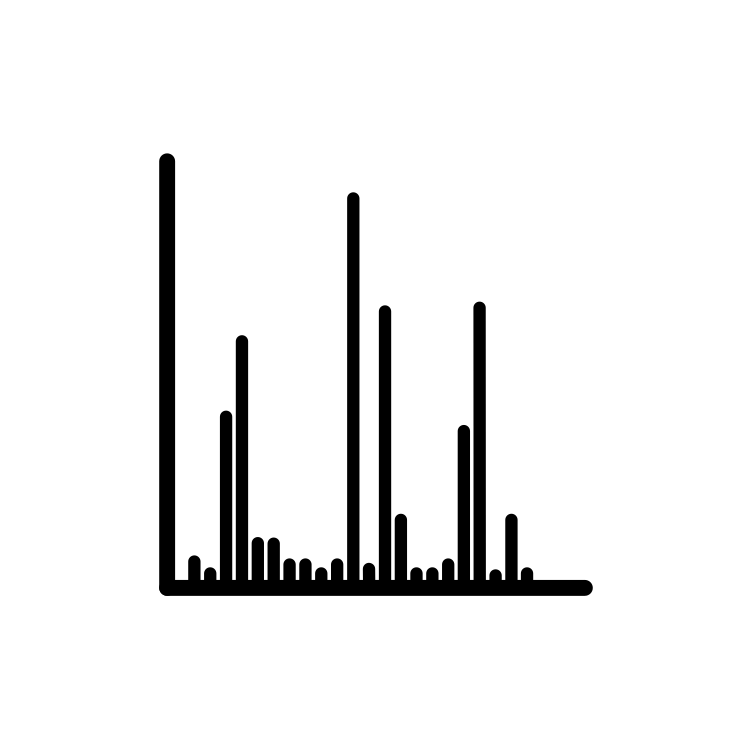
\includegraphics[scale=0.1]{./Presentation_Images/MassSpectraIcon.png}

        \vspace*{-0.4cm}
         $\Downarrow$
         \vspace*{0.2cm}

        \begin{tikzpicture}[scale=0.9]
        \node [circle,draw,ultra thick,color=blue] (0) at (-0.75, 0.75) {};
        \node [circle,draw,ultra thick,color=blue] (1) at (0.25, 1.5) {};
        \node [circle,draw,ultra thick,color=blue] (2) at (-0.25, -0.25) {};
        \node [circle,draw,ultra thick,color=blue] (3) at (0.75, 0.5) {};
        \node [circle,draw,ultra thick,color=blue] (4) at (-1.25, -0.25) {};

        \draw[->,thick] (4) to (0);
        \draw[->,thick] (0) to (2);
        \draw[->,thick] (2) to (3);
        \draw[->,thick] (0) to (1);
        \draw[->,thick] (0) to (3);
        \draw[->,thick] (1) to (3);
        \end{tikzpicture}
  \end{minipage}
            }%
            \onslide<1->{
            \begin{minipage}[c]{0.775\textwidth}
    \begin{itemize}
     \item<1-> Verwendung vorverarbeiteter MS2 Spektren
     \item<1-> Peaks $\rightarrow$ Knoten:
     \begin{itemize}
     \item<2-> \textcolor{\highlightColor}{Peaks} $\widehat{=}$ \textcolor{\highlightColor}{Knotenpaar}
     \item<2-> Knoten bekommen eine \gerquot{Masse}
     \item<2-> Masse $\widehat{=}$ \massCharge Wert
     \item<2-> Startknoten (Masse = 0)
     \item<2-> Endknoten (Masse = Hauptpeak - \emph{M}(\ch{H2O}))
     \end{itemize}
    \end{itemize}
    \end{minipage}
     }%
    \end{frame}

     \begin{frame}{pNovo+ Algorithmus \dashAndSpace Bildung eines Spektrumsgraphen}
               \onslide<1->{
        \begin{minipage}[c]{0.2\textwidth}
        \centering
        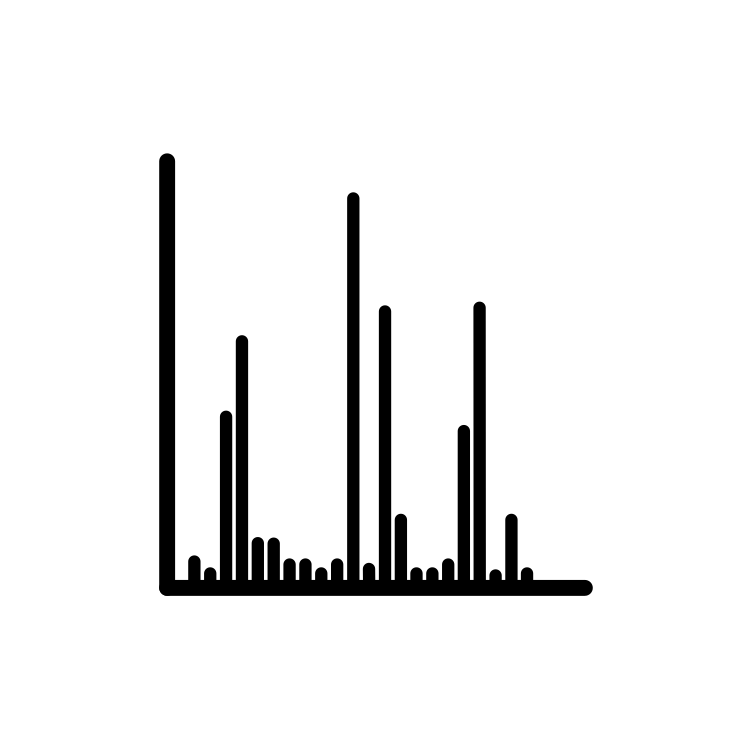
\includegraphics[scale=0.1]{./Presentation_Images/MassSpectraIcon.png}

        \vspace*{-0.4cm}
         $\Downarrow$
         \vspace*{0.2cm}

        \begin{tikzpicture}[scale=0.9]
        \node [circle,draw,thick] (0) at (-0.75, 0.75) {};
        \node [circle,draw,thick] (1) at (0.25, 1.5) {};
        \node [circle,draw,thick] (2) at (-0.25, -0.25) {};
        \node [circle,draw,thick] (3) at (0.75, 0.5) {};
        \node [circle,draw,thick] (4) at (-1.25, -0.25) {};

        \draw[->,ultra thick,color=blue] (4) to (0);
        \draw[->,ultra thick,color=blue] (0) to (2);
        \draw[->,ultra thick,color=blue] (2) to (3);
        \draw[->,ultra thick,color=blue] (0) to (1);
        \draw[->,ultra thick,color=blue] (0) to (3);
        \draw[->,ultra thick,color=blue] (1) to (3);
        \end{tikzpicture}
  \end{minipage}
            }%
            \onslide<1->{
            \begin{minipage}[c]{0.775\textwidth}
      \begin{itemize}
       \item<1-> Gerichtete Kanten zwischen Knotenpaar, wenn:
       \begin{itemize}
        \item<2-> Massendifferenz genau Masse \textcolor{\highlightColor}{einer} AA entspricht
        \item<2-> Massendifferenz genau Masse \textcolor{\highlightColor}{zwei} AA entsprechen
       \end{itemize}
       \item<3-> $N + \binom{n+N-1}{N-1}$ Differenzen ($n=2$, $N=20$)
       \item<3-> \textcolor{\highlightColor}{$230$} Differenzen
      \end{itemize}
      \end{minipage}
      }
     \end{frame}


     \begin{frame}{pNovo+ Algorithmus \dashAndSpace Bildung eines Spektrumsgraphen}
        \begin{itemize}
         \item<1-> Ergebnis: Directed acyclic graph (DAG)
         \item<2-> Beispiel eines Spektrumsgraphen:
        \end{itemize}
\onslide<2->{
\centering
    \begin{tikzpicture}[scale=.7,auto=left,every node/.style={circle,fill=blue!20}]
    \node (begin) at (0,10) {Start};
    \node (end) at (12,10) {End};
    \node (n1) at (2,9) {A};
    \node (n1b) at (2,11) {A};
    \node (n2) at (4,9) {B};
    \node (n2b) at (4,11) {B};
    \node (n3) at (6,9) {C};
    \node (n3b) at (6,11) {C};
    \node (n4) at (8,9) {D};
    \node (n4b) at (8,11) {D};
    \node (n5) at (10,9) {E};
    \node (n5b) at (10,11) {E};

    \tikzset{every node/.style={}}
    \draw[->] (begin) to node[above] {} (n1);
    \draw[->] (n1b) to node[above] {} (n2);
    \draw[->] (n1) to node[above] {} (n2);
    \draw[->] (n1) to[bend right] node[above] {} (n3);
    \draw[->] (n4b) to node[above] {} (n5);

    %\draw[->] (n2) to node[above] {} (n3b);
    \draw[->] (n2) to node[above] {} (n4b);
    \draw[->] (n2) to[bend left] node[above] {} (n4);
    \draw[->] (n4) to node[above] {} (n5);
    %\draw[->] (n1) to[bend right] node[above] {} (n5);
    \draw[->] (n5) to  node[above] {} (end);
    \draw[->] (n5b) to node[above] {} (end);

%   \foreach \from/\to in {begin/n1,n5/end}
%   {
%   \tikzset{every node/.style={}}
%     \draw[->] (\from) -- node[above] {} (\to);
%     }
%     \foreach \from/\to in {n1/n2,n4/n5,n3/n4,n1/n4,n1b/n2}
%   {
%   \tikzset{every node/.style={}}
%     \draw[->] (\from) to[bend left] node[above] {} (\to);
%     }
%     \foreach \from/\to in {n1/n3,n3/n4b,n3/n4,n4/n5}
%   {
%   \tikzset{every node/.style={}}
%     \draw[->] (\from) to[bend right] node[below] {} (\to);
%     }
    \end{tikzpicture}
    }%
    \begin{itemize}
     \item<3-> Alle möglichen Pfade von Start nach End ermitteln
     \item<3-> Scoring Funktion \gerquot{bewertet} jeden Pfad
     \item<3-> Pfad mit dem \textcolor{\highlightColor}{höchsten Scoring Wert} ist das Ergebnis
    \end{itemize}
     \end{frame}

     \begin{frame}{pNovo+ Algorithmus \dashAndSpace Evaluierung}
     \onslide<1->{
        \begin{minipage}[c]{0.2\textwidth}
        \centering
        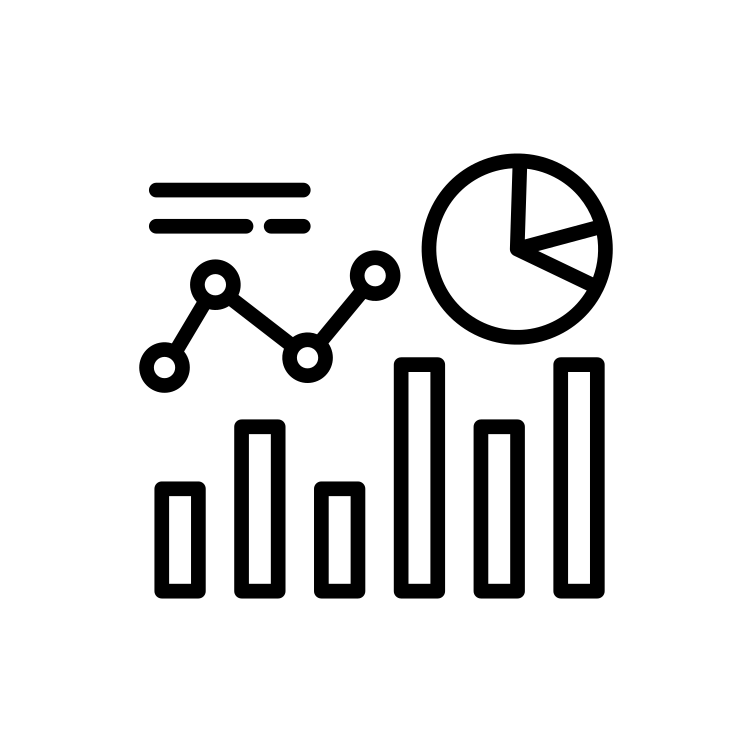
\includegraphics[scale=0.1]{./Presentation_Images/EvaluationIcon.png}
        \end{minipage}
        }%
        \onslide<1->{
        \begin{minipage}[c]{0.775\textwidth}
      \begin{itemize}
       \item<1-> 8677 Datensätze
       \item<1-> Erfolgreiche Sequenzierungen: \textcolor{brown!80!}{$81,2\%$}
       \item<1-> Alternativalgorithmus (PEAKS): \textcolor{orange!75!}{$71.8\%$}
       \end{itemize}
       \vspace*{0.4cm}
       \begin{itemize}
       \item<2-> pNovo+ \textcolor{\highlightColor}{besser als die Konkurrenz!}
       \item<2-> Side Note: pNovo+ ist \textcolor{\highlightColor}{frei verfügbar}
      \end{itemize}
      \end{minipage}
      }
     \end{frame}

    \section{Open-pNovo Algorithmus}
    \begin{frame}{Open-pNovo Algorithmus \dashAndSpace Hintergrund}
     \begin{itemize}
      \item<1-> Peptide sind nicht zwingend stabil
      \item<1-> Wechselwirkungen können die Sequenz abändern
      \item<1-> Posttranslationale Proteinmodifikationenen (PTM)
      % Beispiel einer Wechselwirkung zeigen
      \item<2-> Mit De-Novo-Algorithmen an sich kein Problem ...
      \item<3-> ... wenn nach der Änderung eine AA zurückbleibt
     \end{itemize}
    \end{frame}

    \begin{frame}{Open-pNovo Algorithmus \dashAndSpace PTM}
     \begin{itemize}
      \item<1-> Bildung von nicht proteinogenen AA möglich
      \item<1-> AA, die normalerweise nicht in Peptiden vorkommen
      \item<2-> Spektrogramm zeigt solche AA
      \item<2-> Änderungen können von pNovo+ nicht erkannt werden
      \end{itemize}
      \begin{itemize}
      \item<3-> $\Rightarrow$ pNovo+ erzeugt zwangsweise Fehler
     \end{itemize}
    \end{frame}

      \begin{frame}{Open-pNovo Algorithmus \dashAndSpace RankBoost}
     \begin{itemize}
      \item<1-> Neue Scoring Funktion: RankBoost
      \item<1-> Machine Learning Algorithmus aus 2003
      \item<1-> Erweiterung des AdaBoost Algorithmus
      \item<1-> Präferenzen in Datensätzen zu erkennen
      \end{itemize}
      \begin{itemize}
      \item<2-> Filterung der nicht gültigen AA
     \end{itemize}
    \end{frame}

      \begin{frame}{Open-pNovo Algorithmus \dashAndSpace Evaluierung von Open-pNovo}
      \onslide<1->{
        \begin{minipage}[c]{0.2\textwidth}
        \centering
        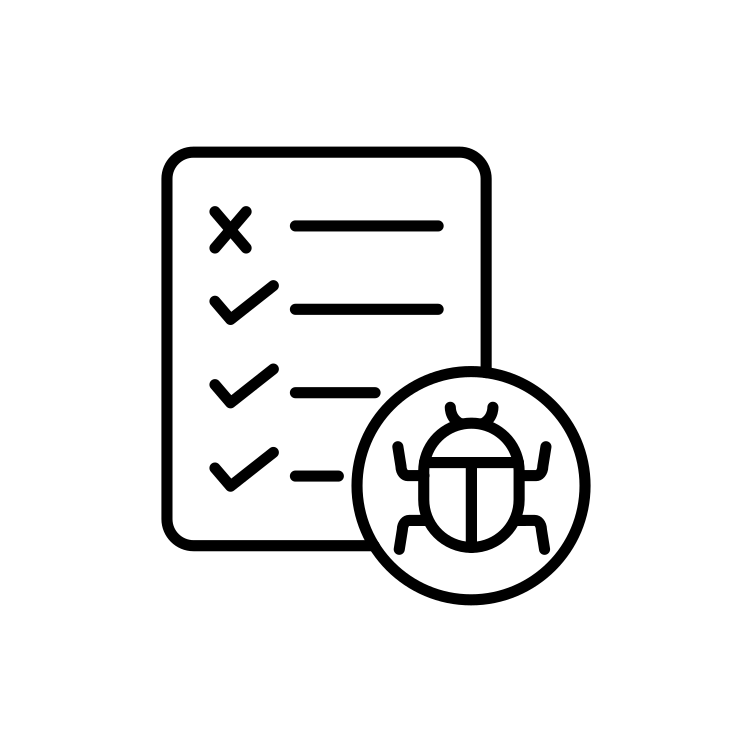
\includegraphics[scale=0.1]{./Presentation_Images/TestingIcon.png}
        \end{minipage}
        }%
        \onslide<1->{
        \begin{minipage}[c]{0.775\textwidth}
     \begin{itemize}
      \item<1-> 45450 Datensätze
      \item<2-> Erfolgreiche Sequenzierungen: \textcolor{brown!80!}{$76,3\%$}
      \item<2-> pNovo+: \textcolor{brown!80!}{$74,5\%$}
      \item<2-> Alternativalgorithmus PEAKS: \textcolor{orange!75!}{$73,1\%$}
      \item<2-> 2. Alternativalgorithmus Novor: \textcolor{orange!75!}{$39,9\%$}
      \end{itemize}
      \vspace*{0.3cm}
      \begin{itemize}
       \item<3-> Verbesserung im Vergleich zu pNovo+
       \item<4-> Allerdings: Weniger als $2\%$ Punkte
       \end{itemize}
       \end{minipage}
       }
    \end{frame}


    \section{Zusammenfassung}
   \begin{frame}{Zusammenfassung}
     \begin{itemize}
     \item<1-> De-Novo-Sequenzierung leichter durchführbar
     \item<1-> Beide Algorithmen liefern \textcolor{\highlightColor}{sehr gute} Ergebnisse
     \item<1-> pNovo+ Ansatz mit Spektrumsgraphen ist wirkungsvoll
      \item<1-> Open-pNovo erkennt zuverlässig Proben mit PTMs
      \vspace*{0.5cm}
      \item<2-> Dennoch: hoher Optimierungsbedarf besteht weiterhin
     \end{itemize}
    \end{frame}

    %%%%% %%%%% %%%%% %%%%% %%%%% BEGIN Ende %%%%% %%%%% %%%%% %%%%% %%%%%
    \begin{frame}{The End}
        \onslide<1->{
            \begin{flushleft}
                \begin{large}
                    \texttt{Danke für die Aufmerksamkeit :)}
                \end{large}
            \end{flushleft}
            \vspace*{0.2cm}
            \begin{flushright}
                \begin{Large}
                    \texttt{Fragen?}
                \end{Large}
            \end{flushright}
        }%
        \onslide<2->{
            \begin{center}
                
\includegraphics[width=0.03\linewidth, angle=-15]{./Presentation_Images/vecteezy_question-mark-with-3d-vector-icon-cartoon-minimal-style_16626300.png}
                
\includegraphics[width=0.04\linewidth]{./Presentation_Images/vecteezy_question-mark-with-3d-vector-icon-cartoon-minimal-style_16626300.png}
                
\includegraphics[width=0.03\linewidth, angle=+15]{./Presentation_Images/vecteezy_question-mark-with-3d-vector-icon-cartoon-minimal-style_16626300.png}
                \\
                \vspace*{0.10cm}
                
\includegraphics[width=0.2\linewidth]{./Presentation_Images/NewTux.png}
            }%
        \end{center}
    \end{frame}
    %%%%% %%%%% %%%%% %%%%% %%%%% BEGIN Ende %%%%% %%%%% %%%%% %%%%% %%%%%

\end{document}
%%%%% %%%%% %%%%% %%%%% %%%%% %%%%% %%%%% %%%%%              %%%%% %%%%% %%%%% %%%%% %%%%% %%%%% %%%%% %%%%%
%%%%% %%%%% %%%%% %%%%% %%%%% %%%%% %%%%% %%%%% END document %%%%% %%%%% %%%%% %%%%% %%%%% %%%%% %%%%% %%%%%
%%%%% %%%%% %%%%% %%%%% %%%%% %%%%% %%%%% %%%%%              %%%%% %%%%% %%%%% %%%%% %%%%% %%%%% %%%%% %%%%%
